\documentclass{article}

% Recommended, but optional, packages for figures and better typesetting:
\usepackage{microtype}
\usepackage{graphicx}
\usepackage{subcaption}
\usepackage{booktabs} % for professional tables
\usepackage{adjustbox}
\usepackage{siunitx}

\usepackage{needspace}


% hyperref makes hyperlinks in the resulting PDF.
% If your build breaks (sometimes temporarily if a hyperlink spans a page)
% please comment out the following usepackage line and replace
% \usepackage{icml2026} with \usepackage[nohyperref]{icml2026} above.
\usepackage{hyperref}


% Attempt to make hyperref and algorithmic work together better:
\newcommand{\theHalgorithm}{\arabic{algorithm}}

% % Use the following line for the initial blind version submitted for review:
\usepackage[accepted]{icml2026}


\usepackage{pgfplots}
\pgfplotsset{compat=1.18}

\usepackage{amsmath}
\usepackage{amssymb}
\usepackage{mathtools}
\usepackage{amsthm}

% if you use cleveref..
\usepackage[capitalize,noabbrev]{cleveref}

% Standard package includes
\usepackage{times}
\usepackage{latexsym}
\usepackage{enumitem}

% For proper rendering and hyphenation of words containing Latin characters (including in bib files)
\usepackage[T1]{fontenc}
% For Vietnamese characters
% \usepackage[T5]{fontenc}
% See https://www.latex-project.org/help/documentation/encguide.pdf for other character sets

% This assumes your files are encoded as UTF8
\usepackage[utf8]{inputenc}

% This is not strictly necessary, and may be commented out,
% but it will improve the layout of the manuscript,
% and will typically save some space.
\usepackage{microtype}

% This is also not strictly necessary, and may be commented out.
% However, it will improve the aesthetics of text in
% the typewriter font.
\usepackage{inconsolata}
\usepackage[scaled=0.85]{helvet}          % sans-serif font


%Including images in your LaTeX document requires adding
%additional package(s)
\usepackage{graphicx}
% \usepackage{amsmath}
\usepackage{xspace}
\usepackage{csquotes}
% Add csquote to xspace exceptions to avoid "text<space>"
\makeatletter
\xspaceaddexceptions{\csq@qclose@i}
\makeatletter
\usepackage{amsfonts}
\usepackage{bbm}
\usepackage{cancel}
\usepackage{caption}
\usepackage{subcaption}
\usepackage{arydshln}


% for unimix vs fasttext chart
\usepackage{pgfplots}
\pgfplotsset{compat=1.18}


% References
% \usepackage{cleveref}
    \crefname{section}{\S}{\S\S}
    \crefformat{section}{\S#2#1#3}
    \crefname{figure}{Fig.}{Fig.}
    \crefname{algorithm}{Alg.}{Alg.}
    \crefname{line}{line}{lines}
    \crefname{appendix}{App.}{}
    \crefname{equation}{eq.}{eqs.}
    \crefformat{equation}{eq.~#2#1#3}
    \crefrangeformat{equation}{eqs.~#3#1#4 to #5#2#6}
    \crefmultiformat{equation}{eqs.~#2#1#3}{ and~#2#1#3}{, #2#1#3}{ and~#2#1#3}
    \crefname{table}{Table}{Tables}
    \crefname{proposition}{Proposition}{Propositions}
    \crefname{assumption}{Assump.}{Assumps.}
    \crefname{definition}{Definition}{Definitions}
    \crefname{theorem}{Thm.}{Thm.}

% Automatic underscore escaping (improved version)
\usepackage{etoolbox} % For \unexpanded
\makeatletter
\DeclareRobustCommand*{\escapeus}[1]{%
  \begingroup
    \edef\x{\endgroup
      \noexpand\@escapeusaux{\unexpanded{#1}}}%
  \x}
\def\@escapeusaux#1{%
  \begingroup
    \@activeus
    \scantokens{#1\endinput}%
  \endgroup}
\begingroup\lccode`\~=`\_
\lowercase{\endgroup
  \def\@activeus{\catcode`\_=\active \let~\_}}
\makeatother

% Makes text sans-serif and automatically escapes "_"
% Way better alternative to monospace
\newcommand{\myemph}[1]{\textsf{{\escapeus{#1}}}}
\newcommand{\vs}{\emph{vs.}\@\xspace}
\newcommand{\eg}{\emph{e.g.}\@\xspace}
\newcommand{\ie}{\emph{i.e.}\@\xspace}
\newcommand{\ngram}{$n$-gram\xspace}
\newcommand{\ngrams}{$n$-grams\xspace}
\newcommand{\R}{\mathbb{R}}
\newcommand{\chspan}[1]{\text{\rmfamily\textit{``#1''}}\xspace}
\newcommand{\size}[1]{{\vert #1 \vert}}
\newcommand{\vect}[1]{\boldsymbol{\mathrm{#1}}}
\newcommand{\softmax}{\mathrm{\text{softmax}}}
\newcommand{\tokenprint}[1]{\text{`#1'}}
% Camera-ready revision marker: wraps every text edit of the 2026-08-09 pass in red for
% author review. To accept all edits, redefine as \newcommand{\camrev}[1]{#1}.
\newcommand{\camrev}[1]{\textcolor{red}{#1}}
% Edits from the special-token correction and the re-release (2026-08-19), kept
% separable from the camera-ready pass above. To accept all, redefine as
% \newcommand{\corrrev}[1]{#1}.
\newcommand{\corrrev}[1]{\textcolor{blue}{#1}}

% Todo note
%\setlength{\marginparsep}{-.2cm}
%\usepackage[textsize=tiny]{todonotes}
\usepackage[disable]{todonotes}
\newcommand{\note}[4][]{\todo[author=#2,color=#3,size=\scriptsize,fancyline,caption={},#1]{#4}} % default note settings, used by macros below
\newcommand{\tiago}[2][]{\note[#1]{\textbf{Tiago}}{cyan!30}{#2}}
\newcommand{\clara}[2][]{\note[#1]{\textbf{Clara}}{orange!30}{#2}}
\newcommand{\Clara}[2][]{\clara[#1,inline]{#2}}
\newcommand{\ahmetcan}[2][]{\note[#1]{\textbf{Ahmetcan}}{yellow!30}{#2}}
\newcommand{\Ahmetcan}[2][]{\ahmetcan[#1,inline]{#2}}
\newcommand{\Tiago}[2][]{\tiago[#1,inline]{#2}}
\newcommand{\pietro}[2][]{\note[#1]{pietro}{green!40}{#2}}
\newcommand{\Pietro}[2][]{\pietro[inline,#1]{#2}}
\newcommand{\response}[2]{\vspace{3pt}\hrule\vspace{3pt}\textbf{#1: }{#2}}
% Macros
\newcommand{\defn}[1]{\textbf{#1}}
% \newcommand{\defeq}{:=}
\newcommand{\defeq}{\mathrel{\stackrel{\textnormal{\tiny def}}{=}}}
\newcommand{\defapproxeq}{\mathrel{\stackrel{\textnormal{\tiny def}}{\approx}}}
\newcommand{\E}{\mathbb{E}}
\newcommand{\addcites}{{\color{red} (add cites)}\xspace}
\newcommand{\done}{{\color{red} (DONE)}\xspace}
\newcommand{\writemore}{{\color{red} ... (write more)}\xspace}
\newcommand{\fasttext}{\myemph{fastText}\xspace}
\newcommand{\unilm}{\myemph{UnigramLM}\xspace}
\newcommand{\glotlid}{\myemph{GlotLID-M}\xspace}
\newcommand{\unilid}{\myemph{UniLID}\xspace}
\newcommand{\cld}{\myemph{CLD3}\xspace}

\newcommand{\likelihood}{\mathcal{L}}
\newcommand{\token}{v}
\newcommand{\stringunit}{s}
\newcommand{\str}{\mathbf{\stringunit}}
\newcommand{\tokens}{\mathbf{\token}}
\newcommand{\stralphabet}{\Sigma}
\newcommand{\stringidx}{t}
\newcommand{\strlength}{|\str|}
\newcommand{\toklength}{M}
\newcommand{\tokindex}{m}
\newcommand{\vocab}{\mathcal{V}}
\newcommand{\corpus}{\mathcal{C}}
\newcommand{\lang}{\ell}
\newcommand{\languages}{\Lambda}
\newcommand{\tokenloss}{\mathrm{loss}}
\newcommand{\pseq}{\mathrm{replace!!}}
\newcommand{\pglobal}{p_{\mathrm{global}}}
\newcommand{\tokenizationfunc}{\mathcal{T}}
\newcommand{\model}{p_{\theta}}
\newcommand{\detokfunc}{\ensuremath{\rotatebox[origin=c]{180}{$\tokfunc$}}}
\newcommand{\tokfunc}{\tau}
\DeclareMathOperator*{\argmin}{\mathrm{argmin}}
\DeclareMathOperator*{\argmax}{\mathrm{argmax}}
\newcommand{\allsegmentations}{\mathcal{T}}
\newcommand{\maxtoklength}{T_{\mathrm{max}}}

\newcommand{\smalldots}{...}
\newcommand{\bpe}{\myemph{BPE}\xspace}
\newcommand{\unigramdist}{\boldsymbol{\phi}}
\newcommand{\unigramdistcur}{\unigramdist^{(n)}}
\newcommand{\tokenprob}{\unigramdist[\token]}


\newcommand{\stringrv}{S_\unigramdist}
\newcommand{\tokenrv}{V_\unigramdist}
\newcommand{\puni}{p_{\unigramdist}}
\newcommand{\pstring}{\puni^S}
\newcommand{\ptokenseq}{\puni^V}
\newcommand{\pZ}{\ptokenseq}   % token-sequence distribution
\newcommand{\pX}{\pstring}   % induced string distribution
\newcommand{\qprior}{q} 
\newcommand{\countv}[2]{c_{#1}(#2)}          
\newcommand{\post}[2]{\puni(#1\,\mid\,#2)} % posterior
\newcommand{\tildec}[2]{\widetilde{c}_{#1}(#2)} 
\newcommand{\hatc}[2]{\widehat{c}_{#1}(#2)} 
\newcommand{\hatcCorpus}[1]{\tildec{#1}{\corpus}} 
\newcommand{\pstringminus}{p^S_{\unigramdist\setminus \token}} 
\newcommand{\joint}[2]{P(\stringrv\!=\!#1, \tokenseqrv\!=\!#2;\unigramdist)} % 

% If the title and author information does not fit in the area allocated, uncomment the following
%
%\setlength\titlebox{<dim>}
%
% and set <dim> to something 5cm or larger.

% \title{What language is this? Ask your tokenizer.}
% % %Other options: 
% % %Speaking in Tokens: UnigramLM for Language ID
% % %LID-as-Tokenization: Using UnigramLM as a Language Identifier

% The \icmltitle you define below is probably too long as a header.
% Therefore, a short form for the running title is supplied here:
\icmltitlerunning{What Language is This? Ask Your Tokenizer.}

\begin{document}

\twocolumn[
  \icmltitle{What Language is This? Ask Your Tokenizer.}
  %Language Identification via Probabilistic Tokenization and Bayesian Inference

  % It is OKAY to include author information, even for blind submissions: the
  % style file will automatically remove it for you unless you've provided
  % the [accepted] option to the icml2026 package.

  % List of affiliations: The first argument should be a (short) identifier you
  % will use later to specify author affiliations Academic affiliations
  % should list Department, University, City, Region, Country Industry
  % affiliations should list Company, City, Region, Country

  % You can specify symbols, otherwise they are numbered in order. Ideally, you
  % should not use this facility. Affiliations will be numbered in order of
  % appearance and this is the preferred way.
  \icmlsetsymbol{equal}{*}

  \begin{icmlauthorlist}
    \icmlauthor{Clara Meister}{epfl}
    \icmlauthor{Ahmetcan Yavuz}{eth}
    \icmlauthor{Pietro Lesci}{camb}
    \icmlauthor{Tiago Pimentel}{eth}
  \end{icmlauthorlist}

  \icmlaffiliation{epfl}{EPFL}
  \icmlaffiliation{camb}{University of Cambridge}
  \icmlaffiliation{eth}{ETH Z\"urich}

  \icmlcorrespondingauthor{Clara Meister}{clara.meister@epfl.ch}
  % \icmlcorrespondingauthor{Firstname2 Lastname2}{first2.last2@www.uk}

  % You may provide any keywords that you find helpful for describing your
  % paper; these are used to populate the "keywords" metadata in the PDF but
  % will not be shown in the document
  \icmlkeywords{Language Identification, Tokenization, Language Modeling}

  \vskip 0.3in
]

% Use ONE of the following lines. DO NOT remove the command.
% If you have no special notice, KEEP empty braces:
\printAffiliationsAndNotice{}  % no special notice (required even if empty)
% Or, if applicable, use the standard equal contribution text:
% \printAffiliationsAndNotice{\icmlEqualContribution}





% \maketitle
\begin{abstract}
Language Identification (LID) is an important component of many multilingual natural language processing pipelines, where it facilitates corpus curation, training data analysis, and cross-lingual evaluation of large language models. Despite near-perfect performance on high-resource languages, existing systems remain brittle in low-resource and closely related language settings.
We introduce \unilid, a simple and efficient LID method based on the \unilm tokenization algorithm, leveraging its probabilistic framing, parameter estimation technique and inference strategy. 
In short, to predict a string's language label, we simply ask: under which language's unigram distribution is this string most likely? 
%In short, we learn language-conditional unigram distributions over a shared tokenizer vocabulary but treat segmentation as a language-specific phenomenon. 
Our formulation is data- and compute-efficient,  supports incremental addition of new languages without retraining existing models, and can naturally be integrated into existing language model tokenization pipelines. Empirical evaluations against widely used baselines, including \fasttext, \glotlid, and \cld, show that \unilid achieves competitive performance on standard benchmarks, substantially improves sample efficiency in low-resource settings---reaching $\sim$70\% accuracy with as few as five labeled samples per language---and delivers large gains on fine-grained dialect identification.\footnote{Implementation at \href{https://github.com/Ahmetcanyvz/UNILID}{github.com/Ahmetcanyvz/UNILID}.}\looseness=-1
\end{abstract}




\section{Introduction}

Language Identification (LID) systems are an important component of today's natural language processing (NLP) landscape. 
They are particularly important for the training and evaluation of large multilingual language models, where they are used to: (i) construct labeled corpora with adequate coverage of the world’s languages, (ii) analyze the composition of large-scale training data,  and (iii) evaluate models' cross-lingual performance. 
As a result, reliable and efficient LID systems have become a vital tool for multilingual language modeling pipelines.


Simple and efficient algorithms have worked well for LID \cite{cavnar01,joulin-etal-2017-bag,lui-baldwin-2012-langid}; many regard it as a \enquote{solved} task since performance on high- and medium-resource languages is often near perfect \cite{mcnamee_solved,lid_survey}. 
However, LID systems often still perform poorly on low-resource languages, closely related language pairs, or fine-grained dialectal distinctions \citep[][\emph{inter alia}]{caswell-etal-2020-language,chifu-etal-2024-vardial,goot-2025-identifying}. 
Even state-of-the-art language models %---despite their strong reasoning and generative capabilities---
fail to consistently identify less common languages \cite{kargaran-etal-2023-glotlid}. 
Collectively, these findings suggest that LID remains far from solved.


In this work, we propose a simple and computationally efficient approach to LID that combines the generative modeling framework underlying the \unilm tokenization algorithm with the classical Bayes decision rule. 
Concretely, \unilm assumes that a string is generated as a sequence of latent subword units drawn independently from a unigram distribution. Rather than learning a single global distribution, we estimate a separate unigram distribution per language. 
Given these language-specific distributions, we approximate the likelihood of an input string in each language using the probability of its most likely subword segmentation under the corresponding unigram model---intuitively, this allows segmentation itself to be treated as a language-dependent latent variable. 
Finally, we apply Bayes’ rule to the resulting language-conditional likelihoods to obtain a posterior distribution over languages, and we assign the language label with the highest posterior probability.
% A direct application of Bayes’ rule to these language-conditional string likelihoods then yields a posterior distribution over languages, and we assign the label that maximizes this posterior. 
%This enables language identification to be carried out as a by-product of tokenization, yielding an interpretable and easily extensible LID system.
% In this work, we propose a simple and computationally efficient method for performing LID. 
% Our approach combines the generative modeling framework underlying the \unilm tokenization algorithm with the classical Bayes decision rule.
% Concretely, we adopt the modeling and estimation procedure of \unilm, in which the data-generating process is represented as a unigram distribution and its parameters are learned from data via the Expectation–Maximization (EM) algorithm \citep{kudo-2018-subword}. 
% Our method makes a fairly indisputable assumption: different languages have different underlying unigram distributions. Accordingly, rather than following the standard \unilm procedure of learning a single unigram model, we learn language-specific token probability distributions over a shared vocabulary. 
% Given these language-conditional distributions, we compute the likelihood of an input string under each language as the probability induced by its most probable segmentation with respect to the corresponding unigram distribution, \ie, we perform the \unilm inference step with per-language distributions. A direct application of Bayes’ rule then yields a posterior distribution over languages, and we assign the label that maximizes this posterior, resulting in a complete language identification system.


The proposed method offers several advantages over prior LID approaches. 
While related to earlier generative LID models \cite{cavnar01,dunning1994statistical}, it departs in a key respect by treating segmentation as a language-specific phenomenon rather than enforcing a fixed tokenization across languages. 
This design choice encourages token boundaries that align with meaningful morphological structure rather than arbitrary statistical artifacts, an approach that is both linguistically motivated and empirically supported in prior NLP work \cite{bostrom-durrett-2020-byte,klein-tsarfaty-2020-getting}.
The per-language distribution formulation further enables incremental extension to new languages or dialects without retraining existing models, and empirically, only a few samples per language are needed to learn language-specific parameters that achieve strong performance. 
Finally, inference is computationally efficient: using clever dynamic programming tricks, inference can be done in an amount of time comparable to the inference step of the classic \unilm tokenization algorithm. %; in practice, the additional pass to compute and compare segmentation probabilities across languages effectively takes $\mathcal{O}(|\languages|)$ time (for language set $\languages$).

% The method\clara{potentially shorten this section} we propose has several distinct advantages over previous approaches.
% While related to earlier generative methods for LID \cite{cavnar01,dunning1994statistical}, our approach differs in a key respect: we treat segmentation itself as a language-specific phenomenon, rather than using fixed segmentation rules across languages. 
% This helps ensure token boundaries align with meaningful morphological units rather than arbitrary statistical artifacts, which is a linguistically-motivated and empirically-validated approach to language modeling \cite{bostrom-durrett-2020-byte,klein-tsarfaty-2020-getting}.\clara{work on sentence} 
% Second, the per-language distribution formulation makes it easy to add new languages or dialects to the label set. 
% No retraining is required for the base vocabulary or existing languages; only the new language’s unigram distribution needs to be learned. 
% Third, training is data- and compute-efficient: empirically, only a few samples per language are needed to learn language-specific parameters that achieve strong performance, while the vocabulary itself can come from any tokenizer---including that of a pretrained language model. 
% Finally, inference is efficient as tokenization accounts for nearly all of the computation required, unlike in other LID methods where it is only a preprocessing step. 
% Specifically, using clever dynamic programming tricks, inference can be done in almost the same time as the inference step of the \unilm tokenization algorithm, requiring only an additional $\mathcal{O}(|\languages|)$ pass (for language set $\languages$) to evaluate and compare segmentation probabilities.\looseness=-1 

Across a diverse set of benchmarks, \unilid achieves performance competitive with widely-used baselines while requiring substantially fewer labeled examples. The method is particularly effective in regimes where LID remains challenging. 
In low-resource settings, \unilid attains $\sim$70\% accuracy with as few as five samples per language and $\sim$90\% accuracy with fewer than 50 samples.
On fine-grained dialect identification, \unilid improves macro F1 from 0.53 to 0.72 relative to a \fasttext baseline. 
Simple post-training calibration steps (calibrated \unilid, \cref{sec:calibration}) raise macro F1 on the 1{,}940-language GlotLID-C test set from \corrrev{.933} to \corrrev{.956}, \camrev{above every system we evaluate on the full GlotLID-C label set (\cref{tab:lid_main})}.
%From a practical perspective, \unilid exhibits substantially shorter training times than \fasttext, while achieving comparable inference throughput, despite using a non-optimized research implementation. 
Taken together, these results suggest that treating segmentation as a language-specific phenomenon provides an effective foundation for language identification.



\newcommand{\lidfunc}{f_\mathtt{lid}}

\section{Language Identification}

Let $\str=\langle\stringunit_1, \dots, \stringunit_T\rangle$ be a string, \ie, a sequence of characters\footnote{The term \enquote{characters} denotes the atomic symbols of the input alphabet, encompassing both Unicode code points and bytes.}
from an alphabet $\stralphabet$, and $\languages$ a set of language labels. 
Closed-set LID is the task of assigning a language $\lang\in\languages$ to $\str$. 
This problem is often framed probabilistically, \ie,
\begin{equation}\label{eq:lang-id}
    \lidfunc(\str) = \argmax_{\lang\in\languages} \,\,p(\lang\mid\str)
\end{equation}
and the task then becomes approximating $p$ with a learned model $\model$. 
Two modeling paradigms are typically employed for solving this task. Discriminative approaches model this distribution using a score $f_\theta(\str,\lang)\in\R$, which is normalized using a softmax function:
\begin{equation}\label{eq:discriminative}
    \model(\lang \mid \str) = \frac{\exp\{f_\theta(\str,\lang)\}}{\sum_{\lang'\in\languages}\exp\{f_\theta(\str,\lang')\}}
\end{equation}
Generative approaches model this distribution via language-conditional likelihoods $\model(\str\mid \lang)$; the desired distribution can then be computed via the Bayes rule:\footnote{We assume a uniform prior over languages in $\languages$ and so drop the explicit $p(\lang)$ term to reduce clutter. }
\begin{equation}\label{eq:bayes}
\model(\lang \mid \str) = \frac{\model(\str \mid \lang)}{\sum_{\lang'\in\languages} \model(\str \mid \lang')}
\end{equation} 
Prior approaches to LID proposed different methods for parameterizing these distributions, as we discuss next.

%SECTION ON CODE SWITCHING; REVISIT GIVEN MORE TIME
% LID is also used in the presence of code-switching. In this case, one considers sequence labeling. Let $\langle x_1,\dots,x_T\rangle$, where $x_t\in\Sigma^*$, be a token or character sequence and $\langle y_1,\dots,y_T\rangle\in\languages^T$ the per-position language labels.\writemore 


\subsection{Prior Approaches}

\paragraph{\ngram Models.} 
Early work on LID established the effectiveness of using plain character-level \ngram statistics with the generative modeling approach of \cref{eq:bayes} \cite{cavnar01,dunning1994statistical}. Explicitly, they estimated language-conditional probabilities with character-level \ngram language models---often augmented with standard backoff or smoothing techniques \citep[\eg, Kneser--Essen--Ney smoothing;][]{kneser}.
%to ensure that the resulting conditional distributions are well-defined and normalized---such as:
% \begin{equation}
% \model(\str\mid\lang) = \prod_{\stringidx=1}^{T} \text{\ngram} \big(\stringunit_\stringidx \,\big|\, \stringunit_{\stringidx-n+1:\stringidx-1}\big)
% \end{equation}
These models set a long-standing baseline for robust LID, particularly on short or noisy texts \cite{Vatanen10LREC,baldwin-lui-2010-language}.

%A canonical example of this approach is \myemph{langid.py} \cite{lui-baldwin-2012-langid}, which uses information gain to identify a small subset of features (specifically byte $n$-grams) that are most effective at distinguishing between languages; it then learns a multinomial Naive Bayes classifier over these features. 

\paragraph{Discriminative Frameworks.}
%Subsequent work explored discriminative frameworks.  %that directly optimize for classification performance given labeled examples. 
In supervised settings, discriminative frameworks often showed improvements over earlier generative approaches, particularly when sufficient training data was available and languages were well represented \cite{lid_survey}.
The standard approach represents input strings as feature vectors encoding character \ngram statistics, such as term-frequency or TF-IDF weights.
Formally, letting $\gamma(\str) \in \R^d$ denote this representation, a linear discriminative model scores each language with $f_\theta(\str, \lang) = \theta_{\lang}^{\top} \gamma(\str)$, instantiating \cref{eq:discriminative}, with $\theta_\lang$ learned by minimizing empirical cross-entropy over labeled data.
A canonical example is \fasttext \cite{joulin-etal-2017-bag}, which averages character $n$-gram embeddings into a single hidden representation and passes it to a linear classifier.
Its architecture is simple, but it has become a standard reference point in LID research: \myemph{OpenLID} and \glotlid pair it with large-scale, curated training data \cite{burchell-etal-2023-open,kargaran-etal-2023-glotlid}, and \myemph{ConLID} \cite{foroutan2025conlid} adds supervised contrastive learning on the same architecture.


% \tiago{This is again a "strong baseline". Descriptions are a bit repetitive in that sense imo. Maybe we can have a sentence in the end saying all are strong baselines? Or say one was replaced by the other. \response{clara}{tried to change this! Lmk what you think :) }}
% Indeed, OpenLID and GlotLID have achieved state-of-the-art coverage and reliability by pairing this architecture with massive, meticulously curated training datasets \cite{burchell-etal-2023-open,kargaran-etal-2023-glotlid}. 


\paragraph{Neural Approaches.} 
In more recent years, neural approaches have been applied to LID. Most are based on character- and byte-level neural sequence models, which arguably provide a more flexible alternative to bag-of-\ngram representations such as \fasttext. Character-level CNN and bidirectional RNN baselines learn feature representations directly from raw text, eliminating the need for explicit feature engineering. % and offering a powerful mechanism for capturing complex orthographic and morphological patterns.
These systems have shown competitive performance, including for streaming or short text LID \cite{zhang_cnn_2015,belinkov-glass-2016-character,kocmi-bojar-2017-lanidenn}.
Google's Compact Language Detector v3 (\cld) uses a shallow feed-forward network over normalized character \ngram frequency features. %\cld has been shown to work particularly well for streaming and short-span settings due to its low-latency design and robustness to very short inputs.
Multilingual Transformer encoders (\eg, mBERT, XLM-R) reach high accuracy with task-specific fine-tuning, but their computational overhead and memory footprint often make them impractical for high-throughput or resource-constrained settings.
 


\subsection{Open Problems}

\paragraph{Varietal and dialectal discrimination.} 
Closely related languages or dialects (\eg, Bosnian, Croatian, and Serbian; Hindi and Urdu; or Maghrebi and Levantine Arabic) have highly similar statistical properties, with a strong overlap in subword-structure and orthography. As a result, even state-of-the-art models struggle with distinguishing between them. Further, there is typically insufficient labeled training data to be able to learn these more fine-grained distinctions \cite{gaman-etal-2020-report,chifu-etal-2024-vardial}.

\paragraph{Low-resource performance.} 
As with many NLP datasets, there exists much more data for a core set of high-resource languages than for the long tail of low-resource ones.
Further, the data that does exist for these low-resource languages is often noisy, \eg, contaminated with HTML code or snippets of text from high-resource languages \cite{kreutzer-etal-2022-quality}.
Parameter estimates for these languages are often poor and, consequently, so is LID performance \cite{caswell-etal-2020-language,kargaran-etal-2023-glotlid}. 
Reweighting, data augmentation, and contrastive objectives have shown promising improvements but have not yet eliminated performance gaps across different resource levels.\cite{ren-etal-2022-effective,burchell-etal-2023-open,foroutan2025conlid}

\paragraph{Domain shift and orthographic noise.} 
Models trained on curated text collections often generalize poorly to informal or domain-mismatched inputs such as social media or transliterated scripts \cite{goot-2025-identifying,ojo2025diversbenchevaluatinglanguageidentification}. Many systems are also not robust to perturbations in orthography (\eg, diacritic omission in languages like French or Vietnamese), as these substantially alter character \ngram statistics, leading to pronounced drops in both accuracy and calibration \cite{caswell-etal-2020-language}.\looseness=-1


\paragraph{This work.} UniLID directly targets the first two challenges. As we show in (\cref{sec:results}), it substantially improves dialect discrimination on DSL-ML 2024 (macro F1 0.53 $\rightarrow$ 0.72) and yields large sample-efficiency gains in the low-resource regime ($\sim$70\% accuracy with five samples per language). On out-of-domain inputs it gives partial improvements (\cref{sec:results}).
%Code-switching and segmentation. Sentence-level classifiers assume monolinguality and misclassify mixed-language inputs. Per-token or per-character labeling with structured decoding improves detection but requires fine-grained supervision and increases computational cost.





\section{UnigramLM}

Tokenization is the process of segmenting strings into sequences of subword units, \ie, character spans referred to as \emph{tokens} in this context. % is the first step in most current NLP pipelines. 
%Current NLP systems begin by segmenting raw strings into sequences of character spans, each mapped to a symbol, known as \emph{token}, in a finite set called \emph{vocabulary}. This process, termed \emph{tokenization}, 
%It determines the basic units a language model uses to process language.\pietro{Updated this section. And stopped for today. Notice how tokens are character spans. I used string only for characters and used "sequence of tokens" and "tokenised string" when referring to a token string. I think this is the right level of detail for this paper. I would not introduce character-string and token-string as we did in tokbias paper. Used emph for less important terms like token and vocab, these are common knowledge. I would use bold for definitions only}
Formally, let $\stralphabet$ be the alphabet of characters $\stringunit$, and $\vocab$ the vocabulary of tokens $\token$. 
Then, tokenization is the mapping of sequences of characters $\str=\langle \stringunit_1,\stringunit_2,\dots\rangle \in\stralphabet^*$ to sequences of tokens 
$\tokens=\langle \token_1,\token_2,\dots\rangle\in\vocab^*$, which we denote as 
$\tokfunc\colon \stralphabet^* \rightarrow \vocab^*$. This mapping is typically injective and thus reversible: the original string can be obtained from its tokenized form through a deterministic detokenization function $\detokfunc\colon \vocab^* \rightarrow \stralphabet^*$, \ie, $\str=\detokfunc(\tokfunc(\str))$. As each token (typically) represents a character span, the definition of $\detokfunc$ is often simple, reducing to concatenating the characters within each token together, \ie: $\detokfunc(\langle\token_1, \token_2, \ldots\rangle) \defeq \token_1 \circ \token_2 \circ \cdots$. 
For example, $\detokfunc(\langle\tokenprint{he},\tokenprint{llo}\rangle) = \chspan{hello}$. Notably, the detokenization function is not necessarily 1-to-1: different token sequences may yield the same string. Reusing the example above, we observe that $\detokfunc(\langle\tokenprint{hell},\tokenprint{o}\rangle)$ still detokenizes to $\chspan{hello}$.
The non-injectivity of $\detokfunc$ is an aspect of tokenization that we will later take advantage of in our LID approach. 
Going forward, we refer to $\tokens$ as a \defn{segmentation} of $\str$ if $\detokfunc(\tokens) = \str$ and define $\allsegmentations_{\vocab}(\str) = \{\tokens : \detokfunc(\tokens) = \str\}$ as the set of all valid segmentations of $\str$ under vocabulary $\vocab$.

Numerous tokenization algorithms exist. 
These algorithms define a mapping function $\tokfunc$ and the method for learning the parameters of this mapping function from data. 
For example, the Byte-Pair Encoding \citep[BPE;][]{sennrich-etal-2016-neural} algorithm defines a $\tokfunc$ parametrized by a list of merges, and a method to learn this list. 
In this work, we focus on the \unilm algorithm \cite{kudo-2018-subword}, which will form the basis of our LID approach.


\subsection{Generative Model}

In broad strokes, \unilm casts tokenization as the uncovering of a latent segmentation: it assumes strings are simply the surface form of a latent sequence of tokens $\tokens$, where each token is drawn independently from a categorical (unigram) distribution.

Let $\unigramdist \in \Delta^{|\vocab|-1}$ denote a probability distribution over a vocabulary $\vocab$, where $\tokenprob$ gives the probability of token $\token$. By construction, $\tokenprob \geq 0$ and $\sum_{\token\in\vocab}\tokenprob = 1$. 
Under the \unilm framework, a token sequence of fixed length $\toklength$ is generated by independently sampling each token from this distribution, and the likelihood of a token sequence $\tokens = \langle \token_1, \smalldots, \token_M\rangle$ is the joint probability of those tokens:\footnote{We would need either an \textsc{eos} token (absorbing state) or a length prior in order to make this a valid probability distribution over $\vocab^*$. This detail is ignored in the standard \unilm implementation, and so we disregard it here as well for faithfulness to the original algorithm.}\clara{@Tiago, would it be correct to say in this footnote also that: in the context of comparing per-language string probabilities, if we assume eos is the same across languages, it would just cancel out? \response{tiago} Hmm, you mean if you assume p(eos) is fixed and constant across languages? Yeah, than I think it's true that it cancels out. Not sure if this is a reasonable assumption though... }
\begin{equation}\label{eq:pZ_single}
    \underset{\text{for}\,\,\tokindex = 1, \ldots, \toklength }{\token_{\tokindex} \stackrel{\text{i.i.d.}}{\sim} \mathrm{Categorical}(\unigramdist)} \, \implies p_{\unigramdist}(\tokens) \defeq \prod_{\tokindex=1}^{|\tokens|} \unigramdist[\token_{\tokindex}] 
\end{equation}
A string $\str$ is then deterministically generated by detokenization. Consequently, the probability of $\str$ is obtained by marginalizing over all valid segmentations:
\begin{equation}
    p_{\unigramdist}(\str) = \sum_{\tokens\in\allsegmentations_{\vocab}(\str)}p_{\unigramdist}(\tokens) 
\end{equation}
which formalizes the data-generating process of a string $\str$ under \unilm's assumptions. 
The posterior distribution over segmentations then follows naturally: %$p_{\unigramdist}(\tokens\mid\str) = p_{\unigramdist}(\tokens)/p_{\unigramdist}(\str)$ for $\tokens \in \allsegmentations_{\vocab}(\str)$ and $0$ otherwise.
\begin{equation}\label{eq:posterior}
    p_{\unigramdist}(\tokens\mid\str) = \frac{p_{\unigramdist}(\tokens)}{p_{\unigramdist}(\str)} \quad \text{for $\tokens \in \allsegmentations_{\vocab}(\str)$ and $0$ otherwise}
\end{equation}

% Given an observed string $\str$, the posterior distribution over token sequences is:
% \begin{equation}
% \label{eq:posterior}
% p_{\unigramdist}(\tokens\mid\str) =
% \begin{cases}
%     &\frac{p_{\unigramdist}(\tokens)}{p_{\unigramdist}(\str)} \quad \text{if } \tokens\in\allsegmentations_{\vocab}(\str)\\
%     &0 \qquad\;\; \text{ otherwise.}
% \end{cases}  
% \end{equation}
Crucially, both  $\unigramdist$ and $\vocab$ are unknown; we only observe the strings resulting from the generative process. The \unilm algorithm estimates these parameters from text data by combining the Expectation–Maximization (EM) algorithm with an iterative vocabulary pruning procedure.


\subsection{Learning Model Parameters}\label{sec:learning-params}

The aim of the procedure proposed by the \unilm algorithm is to find the values of $\unigramdist$ and $\vocab$ that maximize data likelihood. 
Under the \unilm assumptions about the generative process of strings, the \enquote{complete} data consists of $(\str,\tokens)$ pairs, \ie, strings and the sequence of tokens that produced them. 
% Accordingly, our complete dataset looks like $\mathcal{X} = \{(\str_i,\tokens_i)\}_{i=1}^K$ and the \emph{complete}-data log-likelihood is defined as:
% \begin{align}\label{eq:complete-likelihood}
%     \likelihood(\mathcal{X}; \unigramdist) &\defeq  \sum_{i=1}^K\log p_{\unigramdist}(\str_i,\tokens_i)
% \end{align}
Since we only observe strings, and not their underlying segmentations, we cannot directly optimize for \emph{complete}-data log-likelihood; we must instead optimize for the \emph{observed}-data log-likelihood, where the observed data is our text corpus $\corpus=\{\str_k\}_{k=1}^K$:\clara{add something about a prior?}
\begin{equation}\label{eq:corpus-likelihood}
    \likelihood(\corpus; \unigramdist) \defeq \sum_{k=1}^K\,\log\!\!\sum_{\tokens\in \allsegmentations_{\vocab}(\str_k)} p_{\unigramdist}(\tokens) 
\end{equation}
The quantity in \cref{eq:corpus-likelihood} is difficult to optimize directly due to the log-sum structure. The EM algorithm establishes a relationship between this quantity and the expected value of the complete-data log-likelihood, which allows us to solve an easier problem in its stead. 
%To circumvent this issue, \unilm employs the EM algorithm to find unigram probabilities that (approximately) maximize this likelihood.  
In short, the EM algorithm iteratively optimizes parameters with respect to the expected value of the complete data log-likelihood given our observed data $\corpus$ and the distributions induced by our current belief of model parameter values. In the context of \unilm, this boils down to performing the following two steps iteratively until our estimates $\unigramdistcur$ converge:\footnote{$\unigramdist^{(0)}$ can be initialized as \eg, the uniform distribution. See \citet{land2025piecesdoesunigramtokenization} for a discussion of this design choice. }
%
%
\begin{enumerate}[nosep,leftmargin=*]
    \item \textbf{E-Step.} Let $\countv{\token}{\tokens} \defeq \sum_{\tokindex=1}^{|\tokens|}\mathbbm{1}\{\token_\tokindex = \token\}$, \ie, the number of times token $\token\in\vocab$ appears in a segmentation $\tokens$.
    Given current parameters $\unigramdistcur$ and fixed $\vocab$, the E-step computes expected counts in our corpus as
    \begin{equation}
       \hatc{\token}{\corpus;\unigramdistcur}
        \defeq \sum_{k=1}^K 
        \sum_{\tokens\in\allsegmentations_{\vocab}(\str_k)}
        p_{\unigramdistcur}(\tokens \mid \str_k)\; \countv{\token}{\tokens}
    \end{equation}
    This computation is performed using dynamic programming, specifically via the forward-backward algorithm.
    \item \textbf{M-Step.} The M-step then computes the new parameter estimates as simply the normalized expected counts of each token:
    \newcommand{\unigramdistnewtoken}{\unigramdist^{(n+1)}[\token]}
    \begin{equation}\label{eq:mstep}
        \unigramdistnewtoken
        \;=\;
        \frac{\hatc{\token}{\corpus;\unigramdistcur}}
        {\sum_{\token'\in{\vocab}}\hatc{\token'}{\corpus;\unigramdistcur}}.
    \end{equation}
\end{enumerate}

For a proof of\tiago{Is "proof" accurate here? Or would maybe "For a longer exposition on why ..." be better?} why this is a valid approximation of MLE parameters (for a fixed $\vocab$), we refer the reader to the exposition on \unilm in \citet{meister2025unigramlm}.

Intuitively, this procedure resembles maximum likelihood estimation for a categorical distribution, but with a key difference: we cannot compute observed (``hard'') counts of token occurrences, since the segmentation of each string into tokens is latent.  
We instead compute expected (``soft'') token counts under the current model by marginalizing over all possible segmentations. 
%These expected counts are then used to update the unigram parameters. 
In this way, the EM procedure integrates out segmentation uncertainty when estimating $\unigramdist$, yielding parameter estimates that reflect the full distribution over tokenizations rather than a single, fixed segmentation. 


\paragraph{Learning $\vocab$.} 
The EM procedure above operates over a fixed vocabulary $\vocab$. Indeed, the validity of the approximation relies on the fact that $\vocab$ is fixed (and known). 
In the case of our language identification algorithm, we can pre-specify it as, \eg, the vocabulary of a chosen language model. 
If one wishes to also learn the vocabulary, the \unilm algorithm proposes a heuristic approach which works as follows. Initially, $\vocab$ is defined as an oversized set consisting of the most frequently occurring substrings in the corpus; this set can be found efficiently using Enhanced Suffix Array-based algorithms \citep[\eg,][]{Abouelhoda2002TheES}.
The vocabulary is then \enquote{learned} by iterating between: (i) holding it fixed and estimating $\unigramdistcur$ via EM; (ii) a pruning step, where the tokens whose removal hurts corpus log-likelihood the least---under current parameter beliefs $\unigramdistcur$---are removed. 
Via this pruning step, the algorithm ultimately trims the vocabulary down to the user's desired size.\looseness=-1


\subsection{Tokenizing Text}\label{sec:inference}

\newcommand{\unigramdistfinal}{\widehat{\unigramdist}}

At inference time (\ie, when turning text into tokens), the \unilm tokenization algorithm finds the most likely segmentation of $\str$ under the learned parameters $\unigramdistfinal = \unigramdist^{(N)}$ as:\footnote{In the original \unilm algorithm, the most-probable segmentation is chosen rather than the one that has the highest marginal probability. \camrev{We compared both strategies at inference on GlotLID-C: marginalizing scored 0.002 higher macro F1 \corrrev{and the same accuracy to three decimals} (no uncertainty estimate for this comparison) but took \corrrev{roughly 1.7 times as much time} (see \cref{app:viterbi_vs_marginal}).}
%; we therefore use max-probability formulation throughout.
}\looseness=-1%
\begin{subequations}\label{eq:approx-inference}
\begin{align}
    \tokfunc_{\unigramdistfinal}(\str) 
    &\stackrel{\phantom{\text{(\cref{eq:posterior})}}}{=} \argmax_{\tokens \in \vocab^*} p_{\unigramdistfinal}(\tokens\mid\str) \\
    &\stackrel{\text{(\cref{eq:posterior})}}{=} \argmax_{\tokens \in \allsegmentations_{\vocab}(\str)} p_{\unigramdistfinal}(\tokens)\label{eq:drop_strprob}\\
    &\stackrel{\text{(\cref{eq:pZ_single})}}{=} \argmax_{\tokens \in \allsegmentations_{\vocab}(\str)} \prod_{\tokindex=1}^{|\tokens|}\unigramdistfinal[\token_\tokindex] \label{eq:target}
\end{align}
\end{subequations}
% where \cref{eq:drop_strprob} follows from the definition of our posterior and the fact that $p_{\unigramdistfinal}(\str)$ does not depend on $\tokens$ and thus can be dropped.
where we dropped $p_{\unigramdistfinal}(\str)$ in \cref{eq:drop_strprob} since it does not depend on $\tokens$.
The exact solution to \cref{eq:target} can be found efficiently using a Viterbi-style algorithm, which runs in \camrev{$\mathcal{O}(T\cdot \maxtoklength)$ time, where $T$ is the length of the input string $\str$} and $\maxtoklength$ is the length of the longest token $\token\in\vocab$.




\section{\unilid}\label{sec:unilid}

\newcommand{\unigramdistlang}{\widehat{\unigramdist}_{\lang}}
\newcommand{\punigramlang}{p_{\unigramdistlang}}
\newcommand{\unigramdistnewlang}{\unigramdist^{(n+1)}_\lang}

%Framing of LID as a Bayes classifier, where UnigramLM provides our generative model. Application of Bayes rule gives us the probabilty of each language and we choose the max probability one
We propose a generative modeling approach for the LID task using the \unilm framework.
In short, we define language-conditional distributions $\model^{\lang}$ by learning unigram distribution parameters for each language $\lang$, albeit with a shared vocabulary across languages. We then compute language label probabilities, as in  \cref{eq:bayes}, applying the Bayes' decision rule to ultimately assign the language label.

\paragraph{Language-Conditional Distribution Estimation.}
Let $\vocab$ be the vocabulary of a base tokenizer.\footnote{This does not need to be a \unilm tokenizer. Any tokenizer that uses a fixed vocabulary can be used.} 
We fix $\vocab$ as our shared-across-languages vocabulary, but assume there exists, for each language $\lang$, a distinct unigram distribution $\unigramdistlang$ over $\vocab$.
% support across all per-language unigram distributions.
\clara{Is it confusing that we sometimes use 'per-language' and sometimes 'language-conditional'? \response{tiago} So far, I think it's ok. } 
Given a corpus $\corpus^\lang$
%=\{\str_k^\lang\}_{k=1}^{K_\lang}$ 
consisting of strings from language $\lang$, we then learn each of these distributions' parameters $\unigramdistlang$ using the EM procedure described in \cref{sec:learning-params}.\clara{it might be the case that for this problem, we're guaranteed to find the global optimum. Look into that... \response{tiago} Because it's a `simple' distribution? \response{clara}{I guess it would be because of the properties of the objective}}  In other terms, similarly to as in standard \unilm, we compute an approximate maximum likelihood estimate by maximizing the observed-data log-likelihood, albeit on only a subset of the data: 
\begin{equation}
    \unigramdistlang \defapproxeq \argmax_{\unigramdist} \,\,\likelihood(\corpus^\lang; \unigramdist)
\end{equation}
As in the standard \unilm formulation, this procedure integrates over segmentation uncertainty\clara{is this mathematically accurate? \response{tiago} does this mean it marginalises over possible segmentations? I guess it's correct if yes, but a bit of a complicated way of saying that. } when estimating parameters. 
Because data from each language is processed separately, each language gets its own token frequency profile---and consequently its own set of optimal segmentations---despite sharing a common vocabulary across languages. We discuss several design choices we make in our practical implementation of \unilid (\eg, initialization of $\unigramdistlang$ for the EM loop and floor values for token probabilities) in \cref{sec:exp_setup}.

\paragraph{Inference.} At inference time, we use the inference procedure of \unilm discussed in \cref{sec:inference} to find the most probable segmentation of a string under each language's $\unigramdistlang$. 
Importantly, this means that the most probable segmentation $\tokfunc_{\unigramdistlang}(\str)$ can vary across languages. 
This yields a flexible model where the probability of a string reflects language-specific token frequencies, despite sharing a common vocabulary.  
We then approximate the probability of a string under language $\lang$ as the probability of its most probable segmentation in that language: $\model(\str\mid\lang) = p_{\unigramdistlang}(\tokfunc_{\unigramdistlang}(\str))$. Finally, we assign the language label that optimizes the posterior probability, \ie, \cref{eq:lang-id}. We write the instantiation of  \cref{eq:lang-id} here explicitly for the reader's convenience:%
% \begin{subequations}
\begin{align}
    \lidfunc(\str) = \argmax_{\lang\in\languages} p(\lang\mid \str)
   =\argmax_{\lang\in\languages}p_{\unigramdistlang}(\tokfunc_{\unigramdistlang}(\str)) \nonumber
\end{align}
% \end{subequations}

\paragraph{Computational Complexity.}
At training time, \unilid estimates a separate unigram distribution for each language by running the EM procedure over the corresponding language-specific corpus. 
For a corpus $\corpus^\lang$ of total character length \camrev{$T_\lang$} (\eg, number of Unicode code points or bytes), each EM iteration requires computing expected token counts via the forward--backward algorithm, which runs in \camrev{$\mathcal{O}(T_\lang \cdot \maxtoklength)$}, where again $\maxtoklength$ denotes the maximum token length. Parameter updates are linear in the vocabulary size $|\vocab|$. 
Since per-language distribution parameters are estimated independently, training parallelizes trivially across languages. At inference time, \unilid uses a similar Viterbi-style dynamic program as in \unilm:
first building a lattice that enumerates all valid segmentations of a string $\allsegmentations_\vocab(\str)$ and then finding the maximum probability option among them. 
%; we remind the reader that this runs in $\mathcal{O}(N \cdot \maxtoklength)$ time.  
The lattice needs only to be constructed once per string, regardless of the number of language-conditional distributions. 
% Computing the probabilities of segmentations under each language-conditional and f
Finding the optimal segmentation of a string and its probability for each language then takes $\mathcal{O}(|\languages| \cdot E)$ time, where $E$ is the number of edges in the lattice.
% \footnote{The number of edges will be $\mathcal{O}(N\cdot b)$, where $b$ is a branching factor which tells us on average how many tokens in the vocabulary start at position $t$ and are part of a valid segmentation of $\str$ (typically on the order of 1-5 tokens).} 
Finally, we need a $\mathcal{O}(|\languages|)$ pass to evaluate the Bayes decision rule.
The number of edges $E$ in a lattice is \camrev{$T\cdot b$}, where $b$ is the lattice's branching factor, \ie, how many tokens in the vocabulary start at a given string position and are part of a valid segmentation (typically 1-5), so inference takes \camrev{$\mathcal{O}(|\languages|\cdot T\cdot b + T \cdot\maxtoklength)$}.
We compare this cost with \fasttext and \cld in \cref{app:efficiency} and report empirical latency in \cref{sec:results}.


\paragraph{Calibrated \unilid.}\label{sec:calibration}
An error analysis of \unilid on GlotLID-C shows that misclassifications
concentrate on predictions \emph{into} two identifiable groups of languages:
languages with fewer than 18{,}000 training samples, whose estimates
$\unigramdistlang$ remain close to their initialization and therefore assign
moderate probability to strings from many languages, and a group of four
larger languages whose estimated distributions have unusually high entropy
for their script and which \camrev{receive} misclassified samples for the same reason
(the identification criteria are stated in \cref{app:protocol}).
\camrev{On the scored GlotLID-C test pool (\cref{app:protocol}), 32.5\% of
\unilid's false positives (578{,}270 of 1{,}779{,}499) are predictions into
these two groups, whose 1{,}084 languages together hold 3.8\% of the test
lines by gold label.} Both patterns
are symptoms of under-fit distribution estimates. \defn{Calibrated \unilid}
corrects for the two symptoms at inference time; obtaining better estimates
of $\unigramdistlang$ at training time is left to future work.
The first correction makes the treatment of unseen tokens consistent across
languages: the log-probability that language $\lang$ assigns to tokens in
$\vocab$ not observed in $\corpus^\lang$ is \camrev{lowered to one shared
constant wherever it exceeds it,
$\log\unigramdistlang[\token] \defeq \min\bigl(\log\unigramdistlang[\token],\, c\bigr)$
for every $\token$ unseen in $\corpus^\lang$; \corrrev{for the base \unilid
model 1{,}655 of the 1{,}940 unseen-token values lie above $c$ and are set to
$c$; the remaining 285 already lie below $c$ and are unchanged, because the
minimum above never raises a value.}}
\corrrev{Without this correction, that value is the smallest value of
$\log\unigramdistlang$ over $\vocab$, and it varies with the size of
$\corpus^\lang$. Across the 1{,}940 languages, the value decreases by 2.04 nats
for each tenfold increase in the number of training tokens, and the correlation
between the value and $\log_{10}$ of that token count is $-0.99$. For each of
three languages whose corpora were subsampled across two orders of magnitude, the
same decrease per tenfold increase is measured within that one language, so the
quantity that determines the value is corpus size and not the identity of the
language. The training-time
probability floor of $10^{-12}$ does not determine it: every value lies above
that floor, and the smallest distance to it is 7.7 nats.} Since \cref{eq:lang-id} compares
scores across languages, the variation acts as a language-dependent offset on
every unseen token. \camrev{The correction is applied without renormalizing
$\unigramdistlang$, so the corrected per-language values are unnormalized
scores; the decision rule compares them as in \cref{eq:bayes}, and the
posterior interpretation holds up to this approximation.}
The second correction \camrev{re-examines low-margin predictions into} the
two identified groups. Let $s_\lang(\str) = \log
\punigramlang(\tokfunc_{\unigramdistlang}(\str))$ be the score assigned by
language $\lang$ and $\hat\lang = \argmax_\lang s_\lang(\str)$ the
prediction. If $\hat\lang$ belongs to either group and $s_{\hat\lang}(\str)$
exceeds the runner-up score by less than a threshold $\tau_{\hat\lang}$, the
prediction moves to the highest-ranked of the candidates ranked 2 to 5 that
has at least 100{,}000 training samples and a score within 21 natural-log
units of the top candidate; if no candidate qualifies, the prediction is
unchanged. \camrev{Each threshold $\tau_\lang$ is a percentile of the
margins on $\lang$'s own training samples for which $\lang$ is the
top-scoring language, so the threshold bounds the fraction of those samples
that would fall below it; the corresponding statement for test samples is approximate, both
because test margins can differ from training margins and because the
training margins are computed under a distribution estimated from the same
samples.}
\camrev{Each $\tau_\lang$ comes from language $\lang$'s own training
samples. The remaining constants were selected on a validation sample
excluded from every evaluation in this paper and on a development subset of
the scored test pool; the held-out subset behind the confirmation intervals
we report, as well as UDHR, FLORES-200, and CommonLID, entered no constant
selection, with one exception, the $100{,}000$-sample requirement on
replacement candidates, fixed before the development split existed
(\cref{app:protocol} lists which data selected each constant). Because the
development subset is part of the scored pool,
\cref{tab:calibrated_heldout} repeats the comparison of \cref{tab:lid_main}
on the held-out subset alone.} Apart from the high-entropy-group
identification, both corrections depend only on shared constants and on each
language's own data, preserving \unilid's ability to add languages
incrementally.

\section{Experimental Setup}\label{sec:exp_setup}

We evaluate the performance of \unilid across several prominent LID benchmarks.
We note that the majority of our training protocol and evaluation paradigms follow prior work \cite{kargaran-etal-2023-glotlid,foroutan2025conlid}. 
%The choice of benchmarks exhibits the performance of \unilid in high-resource, low-resource, and fine-grained language identification regimes. 
Our experiments compare against widely-used baselines: \fasttext, \cld, and \glotlid. We perform analyses to show data efficiency, robustness to input length, and the impact of using different tokenizer vocabularies.\looseness=-1


\subsection{Datasets}

We choose benchmarks that cover a spectrum of LID regimes, ranging from broad linguistic coverage and low-resource settings to fine-grained dialect identification: GlotLID-C \citep{kargaran-etal-2023-glotlid} for large-scale coverage of
the long tail of nearly 2{,}000 language--script labels;
UDHR \citep{Vatanen10LREC} and FLORES-200 \citep{nllb2022}
for content-controlled cross-lingual evaluation via parallel text across
hundreds of languages;
DSL-ML 2024 \citep{chifu-etal-2024-vardial} for fine-grained dialect
identification across 14 regional varieties with high lexical overlap;
Tatoeba \citep{tiedemann-2020-tatoeba} for robustness on short, noisy,
community-contributed text;
and WiLI-2018 \citep{Thoma2018TheWB} for controlled ablations, as its
balanced 500/500 train/test split across 235 languages supports
controlled comparisons across different dataset stratifications  at
manageable scale. We use official train/test splits where available; full
per-dataset descriptions, including sample counts and split construction,
are deferred to \cref{app:datasets}.
%GlotLID-C \cite{kargaran-etal-2023-glotlid} provides large-scale coverage of the long tail, spanning nearly 2,000 language-script labels with a strong emphasis on low-resource and closely related varieties. UDHR \cite{Vatanen10LREC} and FLORES-200 \cite{nllb2022} consist of parallel text across hundreds of languages, enabling controlled evaluation of cross-lingual performance and generalization independent of semantic content. To assess fine-grained discrimination, we use DSL-ML 2024 \cite{chifu-etal-2024-vardial}, which targets regional and dialectal variants with high lexical overlap. Tatoeba \cite{tiedemann-2020-tatoeba} contains short, user-contributed sentences spanning a large number of languages; texts are often short and noisy, making it an ideal dataset for robustness evaluation.
% Finally, WiLI-2018 \cite{Thoma2018TheWB} is a hallmark LID dataset; it consists of Wikipedia paragraphs with a balanced 500/500 train–test split per language across 235 languages.  
% We use WiLI for our detailed ablations (sample efficiency, input-length effects, and tokenizer-vocabulary comparisons) because it provides a rare combination of (i) a balanced number of examples across all languages, (ii) sufficient per-language data to explore the effect of dataset size while keeping relative dataset language proportions constant\clara{work on wording}, and (iii) manageable scale (235k total examples) that makes repeated controlled experiments feasible. By contrast, GlotLID-C is substantially larger and highly imbalanced across languages, which complicates controlled subsampling studies and makes extensive sweeps prohibitively expensive. 
% Across datasets, we used official train/test splits whenever possible. 


% \setlength{\parskip}{1pt}
\subsection{Baselines}

We compare \unilid against the following systems. For a fair comparison, we hold the training dataset constant across systems that we train ourselves. 
%We indicate for which systems we use pre-trained model checkpoints. 
For systems that did not release reproduction code, or for which we could not reproduce the associated paper's reported performance, we use the released checkpoints. 

\paragraph{\fasttext.} 
We train supervised \fasttext  \cite{joulin-etal-2017-bag} classifiers using the author's Python package\footnote{\href{https://pypi.org/project/fasttext}{\myemph{https://pypi.org/project/fasttext}}.} and following their recommended hyperparameter settings. Models were trained for 100 epochs.\footnote{While the authors' base setup uses fewer epochs, models trained for fewer epochs seriously underperformed on benchmarks. We tuned \fasttext extensively. \camrev{100 epochs gave the best performance in every setting; on DSL-ML 2024 the selection used the shared-task dev split, the same split the dialect results are reported on (no separate validation split exists there), which favors the \fasttext baseline}; see \cref{app:fasttext_epochs} for results on our \fasttext hyperparameter sweep on DSL-ML 2024.}
%\clara{@ahmetcan, can we add just a bit more about that observations here?}.\clara{@ahmetcan can you add a reference to the fasttext library and to whichever work you got the "training recipe" from?}\ahmetcan{Reported training recipes from Conlid and other papers showed 1-2 epoch's are enough but in our trials those epochs seriously underperformed on same benchmarks. To overcome this we tried training for longer and saw significant improvements, after trying different number of epochs we selected 100 epochs as it had acceptable results.}
%\ahmetcan{model comes from pip install fasttext but I also tried C++ build from official repo https://github.com/facebookresearch/fastText}



\paragraph{\cld (pre-trained).} Google's Compact Language Detector v3 (\cld) is a lightweight neural network that supports 107 languages and is optimized for short text segments and low-latency inference. 
%The architecture consists of a feed-forward network that embeds character $n$-grams, averages the embeddings, and passes them through a single hidden layer to a softmax output. 
%It is widely used in commercial settings, motivating its usage as a baseline. 
We use the publicly available pre-trained model from their Python package.\footnote{\href{https://github.com/google/cld3}{\myemph{https://github.com/google/cld3}}.}
%\clara{@ahmetcan can you add a pointer to repo you used?}\ahmetcan{I don't exactly remember it was very hard to run I started from https://github.com/google/cld3 but then I think I used pip install but installing it wasn't straightforward as well}
Its language coverage does not fully overlap with that of our test sets. 
Thus, for a fairer comparison, we provide systems' results computed over only the subset of languages covered by \cld (right side of \cref{tab:lid_main}).

\paragraph{\glotlid (pre-trained).}
\glotlid is the model provided with the GlotLID-C benchmark dataset. Architecturally, it utilizes the \fasttext framework but differentiates itself through its training data curation.  We use their openly available checkpoint, hosted on the same platform as the dataset. 
%\clara{@ahmetcan can you add a pointer to repo you used?} \ahmetcan{https://huggingface.co/cis-lmu/glotlid it is model.bin corresponding to v3 
The exact training splits for \glotlid were not released but the
authors state that UDHR and FLORES-200 are not part of the training
set,\footnote{Their contamination check finds that for 57 languages,
$\leq 10\%$ of UDHR sentences appear in training; see \S3 of
\citet{kargaran-etal-2023-glotlid}.} so we restrict GlotLID-M evaluations
to these two benchmarks.

\begin{table*}[ht]
\centering
\small
\caption{Classification results on benchmark evaluation sets.
\unilid variants and \fasttext are trained using the GlotLID-C corpus.
The left columns show results on the full test sets of each benchmark for models that have full coverage of those benchmark's language label set. The right columns show results on the subsets of the benchmarks that \cld has label coverage for. \camrev{A dash marks a system without coverage of a column's label set; bold marks the best value in a column. The calibrated row (\cref{sec:calibration}) is evaluated on the same test sets.} \corrrev{\Cref{tab:cld3_refit} reports what the full 1{,}940-language \unilid and its calibrated form score on the same benchmark slices. \Cref{app:protocol} states which lines each row was scored on and which models produced the \cld-subset cells.}}
\label{tab:lid_main}
\setlength{\tabcolsep}{5pt}
\renewcommand{\arraystretch}{1.15}
\adjustbox{max width=0.85\textwidth}{
\begin{tabular}{l cc cc cc | cc cc cc}
& \multicolumn{6}{c}{\normalsize \textbf{Full GlotLID-C label set}} &
 \multicolumn{6}{c}{\normalsize \textbf{\cld label set}}\\
\toprule
\textbf{Method} &
\multicolumn{2}{c}{\begin{tabular}[c]{@{}c@{}}\textbf{GlotLID-C test}\\ \small(1940 labels)\end{tabular}} &
\multicolumn{2}{c}{\begin{tabular}[c]{@{}c@{}}\textbf{UDHR}\\ \small(366 labels)\end{tabular}} &
\multicolumn{2}{c}{\begin{tabular}[c]{@{}c@{}}\textbf{FLORES-200}\\ \small(190 labels)\end{tabular}} &
\multicolumn{2}{c}{\begin{tabular}[c]{@{}c@{}}\textbf{GlotLID-C test}\\ \small(83 languages)\end{tabular}} &
\multicolumn{2}{c}{\begin{tabular}[c]{@{}c@{}}\textbf{UDHR}\\ \small(80 languages)\end{tabular}} &
\multicolumn{2}{c}{\begin{tabular}[c]{@{}c@{}}\textbf{FLORES-200}\\ \small(77 languages)\end{tabular}} \\

& F1$\uparrow$ & FPR$\downarrow$
& F1$\uparrow$ & FPR$\downarrow$
& F1$\uparrow$ & FPR$\downarrow$
& F1$\uparrow$ & FPR$\downarrow$
& F1$\uparrow$ & FPR$\downarrow$
& F1$\uparrow$ & FPR$\downarrow$ \\
\midrule

% placeholder1
% & -- & --
% & -- & --
% & -- & --
% & -- & --
% & -- & --
% & -- & -- \\



\cld 
& -- & -- 
& -- & -- 
& -- & -- 
& .906 & 5.48e-4
& .965 & 2.52e-4
& .978 & 2.22e-4 \\

\glotlid
& -- & --
& \textbf{.871} & \textbf{1.37e-4}
& \textbf{.968} & \textbf{1.35e-4}
& -- & --
& .994 & 2.09e-5
& \textbf{.999} & \textbf{6.25e-6} \\

\fasttext
& \camrev{.944} & 2.71e-5
& .855 & 1.87e-4
& .938 & 2.38e-4
& \textbf{.990} & \textbf{7.92e-5}
& \textbf{.998} & 2.98e-5
& .998 & 2.96e-5 \\

\midrule
\unilid
& \corrrev{.933} & \corrrev{2.02e-5}
& \corrrev{.856} & \corrrev{1.52e-4}
& \corrrev{.931} & \corrrev{2.83e-4}
& \corrrev{.974} & \corrrev{1.52e-4}
& \corrrev{.995} & \corrrev{5.73e-5}
& \corrrev{.997} & \corrrev{3.93e-5} \\

\unilid (calibrated, \cref{sec:calibration})
& \corrrev{\textbf{.956}} & \camrev{\textbf{1.77e-5}}
& \corrrev{.842} & \corrrev{2.03e-4}
& \corrrev{.932} & 2.91e-4
& \corrrev{.981} & \corrrev{1.48e-4}
& \corrrev{.993} & \corrrev{7.57e-5}
& \corrrev{.997} & \corrrev{3.29e-5} \\

\unilid-Mistral-Nemo
& .912 & \camrev{1.84e-5}
& .836 & 1.79e-4
& .923 & 3.22e-4
& .972 & 1.53e-4
& .992 & \camrev{1.03e-4}
& .994 & 8.05e-5 \\

\unilid-DeepSeek3.2
& .909 & 2.08e-5
& .836 & 1.78e-4
& .914 & 3.42e-4
& .971 & 1.66e-4
& .990 & 1.33e-4
& .994 & 7.92e-5 \\

\unilid-Qwen3
& .904 & 2.55e-5
& .829 & 1.91e-4
& .904 & 3.80e-4
& .964 & 2.27e-4
& .984 & 2.11e-4
& .989 & 1.46e-4 \\





\bottomrule
\end{tabular}}
\end{table*}



\subsection{Evaluation Metrics}


% We focus on the macro-averaged F1 score and false positive rate (FPR), defined as
% \begin{equation}
%     \mathrm{F1} = \frac{1}{|\languages|} \sum_{\lang \in \languages} \frac{2 \cdot \mathrm{P}_{\lang} \cdot \mathrm{R}_{\lang}}{\mathrm{P}_{\lang} + \mathrm{R}_{\lang}},\,\, \mathrm{FPR} = \frac{1}{|\languages|} \sum_{\lang \in \languages} \frac{\mathrm{FP}_{\lang}}{\mathrm{FP}_{\lang} + \mathrm{TN}_{\lang}}
% \end{equation}
% where $\mathrm{P}_{\lang}$ and $\mathrm{R}_{\lang}$ denote the precision and recall for language $\lang$, and $\mathrm{FP}_{\lang}$ and $\mathrm{TN}_{\lang}$ denote the number of false positives and true negatives, respectively.
%  Macro-averaging ensures that performance across each language/dialect contributes equally to the overall score.  
% For data efficiency and robustness analyses on WiLI, we additionally report classification accuracy.
% These are the standard metrics of focus in LID.\looseness=-1
We report standard evaluation metrics for language identification, namely the macro-averaged F1 score and the macro-averaged false positive rate (FPR)\camrev{, defined as}
{\color{red}\begin{equation}
    \mathrm{F1} = \frac{1}{|\languages|} \sum_{\lang \in \languages} \frac{2 \cdot \mathrm{P}_{\lang} \cdot \mathrm{R}_{\lang}}{\mathrm{P}_{\lang} + \mathrm{R}_{\lang}},\,\, \mathrm{FPR} = \frac{1}{|\languages|} \sum_{\lang \in \languages} \frac{\mathrm{FP}_{\lang}}{\mathrm{FP}_{\lang} + \mathrm{TN}_{\lang}}
\end{equation}}%
\camrev{where $\mathrm{P}_{\lang}$ and $\mathrm{R}_{\lang}$ denote the precision and recall for language $\lang$, $\mathrm{FP}_{\lang}$ counts the test samples of other languages predicted as $\lang$, and $\mathrm{TN}_{\lang}$ counts the test samples of other languages not predicted as $\lang$.} Macro-averaging ensures that each language or dialect contributes equally to the overall score, regardless of class frequency. For analyses of data efficiency and robustness on the WiLI dataset, we additionally report classification accuracy.

\subsection{\unilid Training}
For each benchmark, we learn language-conditional unigram distributions using the EM procedure of the \unilm tokenization algorithm, described in \cref{sec:learning-params}.  
In all experiments, we initialize the unigram distribution as the uniform distribution and run EM for $20$ rounds.\footnote{We observed empirically that unigram distributions always converged within 20 rounds (\ie, the total variation distance between subsequent rounds fell below $10^{-6}$).}\clara{Footnote comment: could also use the SentencePiece settings to justify $\leq 20$ rounds if that would make the argument stronger \response{tiago} I think saying it converged is enough. Also, it's our own method and not a baseline, so maybe we don't need to motivate it as much as for baselines? (I mean if our own method underperforms a bit at these settings, it's not really a big issue.)} 
To avoid zero-probability segmentations when a token's expected counts are estimated to be 0 under a given language (most common in the few-sample regime), we floor token probabilities at $10^{-12}$ during training. For calibrated \unilid (\cref{sec:calibration}) we use the shared unseen-token constant \corrrev{$c = -17$} (natural log).
%, re-examine predictions into languages with fewer than 18{,}000 training samples (and four large-corpus languages with unusually flat token distributions), 
We set each margin threshold $\tau_\lang$ at the $q_\lang = 5\,(1 - N_\lang/18{,}000)$ percentile of language $\lang$'s own training margins for the languages below 18{,}000 samples, and at a fixed 5th percentile for the four high-entropy languages of \cref{sec:calibration}.
The full protocol, remaining constants, and their provenance are in \cref{app:protocol}.
We consider two variants of \unilid: one that uses a dedicated base tokenizer trained on the LID training set, and one that uses the vocabulary of a pretrained language model; more details below.

\paragraph{\unilid.}
The base version of \unilid trains a tokenizer on the training split of each benchmark dataset\camrev{; for GlotLID-C, the base tokenizer is trained on a subsample of 1{,}000 samples per language (\cref{tab:training_time})}. We train a byte-level tokenizer using the standard \unilm tokenization algorithm. Our implementation closely follows the design choices of the SentencePiece library \cite{kudo-richardson-2018-sentencepiece}, which provides the original implementation of \unilm. Unless otherwise specified, we use a vocabulary size of $100\text{k}$; ablation experiments indicate that performance is relatively insensitive to this choice (see \cref{sec:ablations}).\clara{potentially add details of pretokenization choices: ByteLevel(add\_ prefix\_space=True, use\_regex=True)}


%For the WiLI benchmark, we use the full training set of texts as the base tokenizer training data.
%For benchmarks with highly unbalanced dataset splits, e.g., GlotLID-C, we cap the number of strings per language to $100k$.\looseness=-1

\paragraph{\unilid-X.}
This variant uses the vocabulary of a pretrained base tokenizer and learns only the per-language unigram distributions. 
This setting evaluates \unilid’s ability to operate with pretrained, task-agnostic vocabularies. 
We report results using the \myemph{Mistral-Nemo-Base-2407}\footnote{\href{https://huggingface.co/mistralai/Mistral-Nemo-Base-2407}{\myemph{https://huggingface.co/mistralai/Mistral-Nemo-Base-2407}}.} tokenizer \cite{mistral}, which we refer to as \unilid-Mistral-Nemo. Results obtained with other base tokenizers, which yield comparable performance, are reported in \cref{sec:ablations}.




% \begin{figure}[t]
%     \centering
%     \adjustbox{max width=\linewidth}{
%     \begin{tikzpicture}
%     \begin{axis}[
%         width=\linewidth,
%         height=0.45\linewidth,
%         grid=both,
%         symbolic x coords={5,10,25,50,100,200,300,400,500},
%         xtick={5,10,25,50,100,200,300,400,500}, 
%         enlarge x limits=0.05,
%         ymin=0, ymax=100,
%         xlabel={Samples per Language},
%         ylabel={Accuracy (\%)},
%         legend pos=south east,
%         legend cell align=left,
%         tick align=outside
%     ]
%     % FastText
%     \addplot+[mark=*, line width=0.9pt]
%     coordinates {
%         (5,0.10) (10,0.01) (25,13.74) (50,67.55) (100,85.91)
%         (200,91.77) (300,92.22) (400,94.01) (500,94.55)
%     };
%     \addlegendentry{\fasttext}
    
%     % UnimixLM
%     \addplot+[mark=square*, line width=0.9pt]
%     coordinates {
%         (5,70.20) (10,79.37) (25,88.72) (50,92.66) (100,94.13)
%         (200,95.04) (300,95.31) (400,95.52) (500,95.65)
%     };
%     \addlegendentry{\unilid}
%     \end{axis}
%     \end{tikzpicture}}
%     \caption{Sample efficiency analysis  on WiLI: \unilid maintaxins $>70\%$ LID accuracy with only 5 samples per language, whereas \fasttext requires 50+ samples to reach comparable performance.}
%     \label{fig:samples-accuracy}
% \end{figure}



\begin{table*}[t]
\centering
\small
\caption{Per-dialect and macro-averaged F1 scores on the DSL-ML 2024 task for French (FR), Spanish (ES), Portuguese (PT), English (EN), and the Bosnian/Croatian/Montenegrin/Serbian family.}
\label{tab:per_language_f1}
\setlength{\tabcolsep}{4pt}
\renewcommand{\arraystretch}{1.15}
\adjustbox{max width=0.7\textwidth}{
\begin{tabular}{l *{4}{c} | *{2}{c} | *{2}{c} | *{2}{c} | *{4}{c} | c}
\toprule
& \multicolumn{4}{c}{\textbf{French}} & \multicolumn{2}{c}{\textbf{Spanish}} & \multicolumn{2}{c}{\textbf{Portuguese}} & \multicolumn{2}{c}{\textbf{English}} & \multicolumn{4}{c}{\textbf{BCMS}} & \\
\cmidrule(lr){2-5} \cmidrule(lr){6-7} \cmidrule(lr){8-9} \cmidrule(lr){10-11} \cmidrule(lr){12-15}
\textbf{Model} & BE & FR & CA & CH & ES & AR & BR & PT & US & GB & SR & HR & BS & ME & \textbf{Macro} \\
\midrule
\unilid & .595 & .288 & .798 & \textbf{.456} & \textbf{.867} & \textbf{.832} & \textbf{.816} & \textbf{.724} & \textbf{.855} & \textbf{.815} & \textbf{.929} & \textbf{.788} & \textbf{.609} & \textbf{.750} & \textbf{.723} \\
\fasttext & \textbf{.697} & \textbf{.434} & \textbf{.811} & .444 & .833 & .686 & .729 & .609 & .815 & .561 & .833 & .000 & .000 & .000 & .532 \\
\bottomrule
\end{tabular}%
}
\end{table*}


\begin{table}[t]
\centering
\small
\caption{Macro-averaged F1 and false positive rate (FPR) of \fasttext and \unilid trained on WiLI and evaluated on the Tatoeba and UDHR benchmarks.}
\label{tab:tatoeba_udhr_comparison}
\setlength{\tabcolsep}{7pt}
% \renewcommand{\arraystretch}{1.}
\adjustbox{max width=\linewidth}{
    \begin{tabular}{lcccc}
    \toprule
    \textbf{Method} &
    \multicolumn{2}{c}{\textbf{Tatoeba} (201 langs)} &
    \multicolumn{2}{c}{\textbf{UDHR} (142 langs)} \\
    & \textbf{Macro F1}$\uparrow$ & \textbf{Macro FPR}$\downarrow$
    & \textbf{Macro F1}$\uparrow$ & \textbf{Macro FPR}$\downarrow$ \\
    \midrule
    \fasttext & 0.160 & 3.58e-3 & 0.849 & 6.07e-4 \\
    \unilid & \textbf{\corrrev{0.420}} & \textbf{\corrrev{9.23e-4}} & \textbf{\corrrev{0.866}} & \textbf{\corrrev{5.86e-4}} \\
    \bottomrule
    \end{tabular}%
}
\end{table}


\section{Results}\label{sec:results}

\paragraph{Base Results.} 
We first evaluate \unilid on standard LID benchmarks: GlotLID-C, UDHR, and FLORES-200. Although \unilid is not always the top-performing system in terms of F1, \cref{tab:lid_main} shows that both \unilid and \unilid-Mistral-Nemo achieve competitive macro-averaged F1 scores while consistently maintaining low FPR across both large-scale settings and low-resource datasets. 
Notably, on the largest evaluation set (full GlotLID-C test), \unilid reduces FPR by roughly 25\% compared to \fasttext (\corrrev{2.02e-5} vs 2.71e-5)---a property that can be more critical than F1 in many LID applications. For example, in web-scale crawling, a poor FPR for a low-resource language can lead to a training corpus dominated by noise (common languages misclassified as rare ones). 
%the erroneous assignment of data to a low-resource language is essential.
%, minimizing the risk of false positives in large-scale filtering pipelines. 
Overall, these results demonstrate \unilid’s efficacy as a general-purpose LID system.
In subsequent sections, we compare primarily against \fasttext. It is the only of these systems for which we can control training data (\glotlid is an instantiation of \fasttext, just with a particular dataset); we cannot control for test-set contamination or sample efficiency with the other systems.


\paragraph{Effect of Calibration.}
On GlotLID-C, calibrated \unilid (\cref{sec:calibration}) raises macro F1
from \corrrev{0.933} to \corrrev{0.956}, above every system in \cref{tab:lid_main} with full
GlotLID-C label coverage, while
lowering macro FPR from \corrrev{2.02e-5} to 1.77e-5; on a held-out subset outside
every calibration-constant selection \camrev{except the $100{,}000$-sample
requirement}
(\cref{app:protocol}), the paired bootstrap interval of the
improvement over \unilid is \corrrev{$+0.034$} with 95\% interval \corrrev{$[+0.029, +0.038]$}
(\cref{tab:calibrated_heldout}). \camrev{The gain sits where
\cref{tab:calibrated_views} reports \unilid's weakness: under the view in
which every false positive counts against the predicted language, mean
per-language F1 rises from \corrrev{0.596} to \corrrev{0.781} for languages with fewer than 500
training samples, and from \corrrev{0.676} to \corrrev{0.893} for languages with 500 to 1{,}000
training samples (scored GlotLID-C test pool).} \camrev{The gains are
specific to test data whose per-language line counts follow the
collection's natural imbalance, where false-positive volume into
under-resourced languages matters: on the parallel, equal-support UDHR set
(366 labels, many of them under-resourced) calibration lowers macro F1
(\corrrev{0.856} to \corrrev{0.842}), while FLORES-200 (190 labels, mostly larger languages)
changes little (\corrrev{0.931} to \corrrev{0.932}); \cref{app:protocol} reports the
balanced-draw measurement of the same effect.}
On out-of-domain web-domain data (CommonLID, \cref{tab:commonlid}),
calibration raises macrolanguage-aware accuracy from \corrrev{0.848} to \corrrev{0.862}\camrev{,
while tag-level macro F1 moves from \corrrev{0.722} to \corrrev{0.717}}. The
re-examination touches few lines on benchmarks of larger languages: on
FLORES-200 it examines 1{,}484 of 192{,}280 lines and moves 799.

%\Ahmetcan{On dslml we didn't use sentencepiece because it gives an error on dslml we use your custom EM method, Also updated numbers}
\paragraph{Dialect Differentiation.}
\cref{tab:per_language_f1} reports results on the DSL-ML 2024 benchmark. 
\unilid demonstrates strong performance in comparison to participant submissions in the DSL-ML 2024 shared task. On French dialects, \unilid achieves a macro-F1 of 0.534 in comparison to 0.385 for the top shared-task system.  \unilid provides smaller but consistent gains on the other dialect groups as well:  Spanish (0.850 vs 0.823), Portuguese (0.770 vs 0.752), and BCMS (0.769 vs 0.762). 
It also substantially outperforms \fasttext on macro F1, improving from 0.53 to 0.72. We note that part of this result is driven by the 0.00 F1 achieved by \fasttext on several of the Slavic languages. This poor performance may in part be due to the small amount of training data for those languages (see \cref{app:datasets} for the dataset breakdown), a regime that \cref{fig:samples-accuracy} likewise evinces that \fasttext struggles with. 
There are several potential reasons why \unilid  performs particularly well in this regime: First, UniLID's vocabulary $\vocab$ provides a structural inductive bias; only per-language token frequencies must be estimated from the data. This stands in contrast to setups like \fasttext, where high-dimensional embeddings for millions of $n$-gram spans must be adjusted to give signal for the language. Second, generative classifiers are known to be more sample-efficient than discriminative ones in low-data regimes \cite{ng2001discriminative}, and UniLID is generative while fastText is discriminative.


%---one characterized by high lexical overlap and minimal orthographic differences---supports the hypothesis that treating segmentation as language-specific provides a meaningful advantage in fine-grained classification settings.


\begin{figure}[t]
    \centering
    \adjustbox{max width=0.8\linewidth}{
    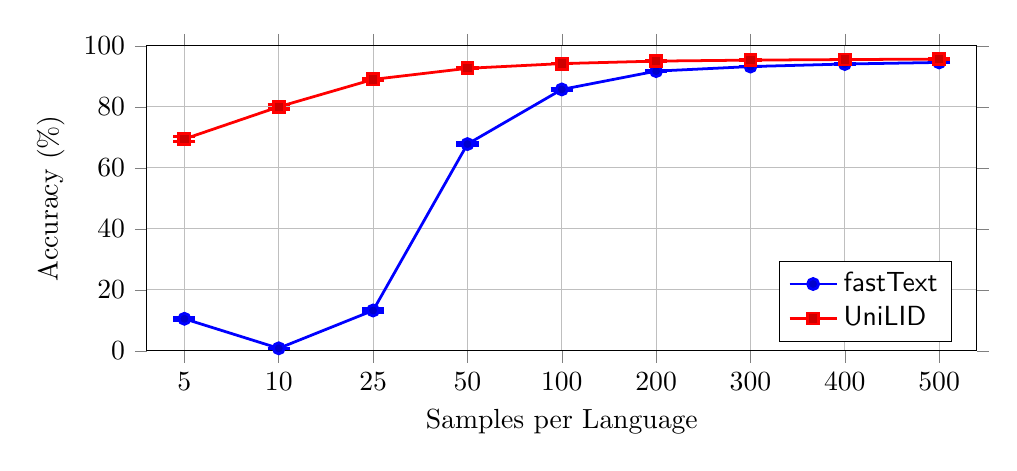
\begin{tikzpicture}
    \begin{axis}[
        width=\linewidth,
        height=0.45\linewidth,
        grid=both,
        symbolic x coords={5,10,25,50,100,200,300,400,500},
        xtick={5,10,25,50,100,200,300,400,500}, 
        enlarge x limits=0.05,
        ymin=0, ymax=100,
        xlabel={Samples per Language},
        ylabel={Accuracy (\%)},
        legend pos=south east,
        legend cell align=left,
        tick align=outside,
    ]

    % ---------------- FastText ----------------
    \addplot+[
        mark=*,
        line width=1pt,
        error bars/.cd,
            y dir=both,
            y explicit,
            error bar style={line width=1.2pt},
            error mark options={
                rotate=90,
                mark size=4pt,
                line width=1.2pt
            },
    ]
    coordinates {
        (5,10.53) +- (0,0.43)
        (10,0.85) +- (0,0.00)
        (25,13.25) +- (0,0.53)
        (50,67.79) +- (0,0.52)
        (100,85.70) +- (0,0.40)
        (200,91.70) +- (0,0.04)
        (300,93.20) +- (0,0.04)
        (400,94.03) +- (0,0.03)
        (500,94.55) +- (0,0.06)
    };
    \addlegendentry{\fasttext}

    % ---------------- UniLID ----------------
    \addplot+[
        mark=square*,
        line width=1pt,
        error bars/.cd,
            y dir=both,
            y explicit,
            error bar style={line width=1.2pt},
            error mark options={
                rotate=90,
                mark size=4pt,
                line width=1.2pt
            },
    ]
    coordinates {
        (5,69.46) +- (0,0.90)
        (10,80.01) +- (0,0.68)
        (25,88.99) +- (0,0.34)
        (50,92.62) +- (0,0.14)
        (100,94.17) +- (0,0.06)
        (200,94.99) +- (0,0.02)
        (300,95.31) +- (0,0.03)
        (400,95.50) +- (0,0.02)
        (500,95.64) +- (0,0.00)
    };
    \addlegendentry{\unilid}

    \end{axis}
    \end{tikzpicture}}
    \caption{Sample efficiency analysis on WiLI (mean $\pm$ std). \unilid achieves substantially higher accuracy in the low-resource regime while maintaining consistently low variance across runs.}
    \label{fig:samples-accuracy}
\end{figure}

\paragraph{Low-resource Regime.}
We evaluate sample efficiency on WiLI by varying the training dataset size.\tiago{Table 1 seems to have quite mixed results, but all the extra experiments are on Wili in which we seem quite better. So maybe justifying why wili could be nice?}
Concretely, we train each model on a subset of the WiLI training set, created by taking $K$ points from each language set. \textit{E.g.}, at $K=5$, there are a total of $5\times |\languages|$ data points in the entire training set; training subsets are the same for each model at a given value of $K$. 
\cref{fig:samples-accuracy}\tiago{Table 4 currently appears before Table 3. Maybe we should switch their order.} shows system accuracy as a function of $K$.  
Results show that \unilid dramatically outperforms \fasttext\footnote{We tuned \fasttext extensively for this setting but could not improve performance; the best configuration is reported here, with a subset of our sweep of \fasttext hyperparameters in \cref{app:fasttext_epochs}. } in the low-resource regime. 
With as few as 5 samples per language, \unilid achieves $\sim$70\% accuracy, while \fasttext fails to generalize. 
Performance remains strong even with fewer than 50 samples per language, highlighting the strength of \unilid in scenarios in which labeled data is scarce or expensive to obtain.
We provide the values displayed in \cref{fig:samples-accuracy} in \cref{tab:samples-accuracy} in \cref{app:additional_results}.

\paragraph{Out-of-domain Performance.}
\cref{tab:tatoeba_udhr_comparison} evaluates generalization by training on Wikipedia (WiLI) and testing on short, noisy community-contributed text (Tatoeba) and formal legal documents (UDHR). 
\unilid demonstrates superior domain robustness, \emph{more than doubling} the Macro F1 of \fasttext on Tatoeba (\corrrev{0.420} vs. 0.160).
%While performance drops compared to in-domain evaluation, \unilid achieves strong performance on UDHR relative to the \fasttext baseline. 
These results evince the generalization abilities of the \unilid approach, particularly for short, informal inputs, which is a domain in which current SOTA systems struggle.






\paragraph{Robustness Analysis.}
\cref{tab:length_accuracy} reports accuracy as a function of input length on WiLI. 
\unilid consistently outperforms \fasttext across all length buckets, with the largest gains observed for shorter inputs, which is a regime in which most LID systems struggle. 
This highlights the robustness of \unilid's language-specific segmentation assumptions for low-context settings, which are common in practical LID applications, such as determining the language of social media posts.

\paragraph{Vocabulary Sensitivity.}
\cref{tab:lid_main} includes three UniLID-X variants that reuse off-the-shelf LLM tokenizer vocabularies (Mistral-Nemo, DeepSeek-3.2, Qwen-3); all are \corrrev{within 0.03 macro F1}
of base UniLID on GlotLID-C, with similar behavior for other LLM
tokenizers (\cref{app:additional_results}).
The gap in F1 is not negligible though. Clearly, training the base \unilid tokenizer on broad multilingual data, such that it attains a comprehensive multilingual vocabulary, does lead to better performance---both in-distribution (e.g., GlotLID-C train $
\rightarrow$ GlotLID-C test) and out-of-distribution (GlotLID-C train $\rightarrow$ UDHR, FLORES-200, neither of which appears in the training set; see \cref{tab:lid_main}).  
LLM tokenizers, on the other hand, are optimized for general-purpose language modeling on data distributions that under-represent the low-resource tail of GlotLID-C.  We
accordingly recommend, for production deployment, training the base
tokenizer once on a broad, web-representative multilingual corpus, and
then estimating per-language unigram distributions incrementally as data
for new languages arrives. \unilid-X is intended as a convenience mode for practitioners who wish to reuse an existing LLM tokenizer or to integrate LID into an existing LLM tokenization pipeline at no additional vocabulary cost.
We additionally explore the effect of vocabulary size in \cref{app:additional_results}. 
%: training base tokenizers with vocabularies ranging in size from 10$k$ to 200$k$ tokens. 
Performance improves modestly with increasing vocabulary size before plateauing, suggesting that UniLID is relatively robust to this choice and does not require extremely large vocabularies to perform well.



\paragraph{Efficiency.} \camrev{\cref{app:efficiency}}
reports inference latency and wall-clock training time for \unilid, \fasttext, and \cld measured on identical hardware. Training UniLID on the full
GlotLID-C corpus (1{,}940 language--script classes) takes 17.8k seconds
end-to-end versus $\sim$163k seconds for the 100-epoch \fasttext
configuration, an approximately $9\times$ reduction despite our
unoptimized research implementation\camrev{; the comparison is conditioned
on the 100-epoch configuration, which was selected for accuracy (at 1 epoch
\fasttext reaches macro F1 0.115 on DSL-ML 2024, against 0.532 for the
configuration used in this paper; \cref{tab:fasttext_epoch_sweep})}.
Inference latency varies with the
label set size: on GlotLID-C (1{,}940 labels), \unilid is \camrev{$1.85\times$ slower
than \fasttext (0.307 vs 0.166 ms/sample) and $1.64\times$ slower than
\cld (0.187 ms/sample); on WiLI (235 labels), UniLID is the second-fastest
of the three (0.155 ms/sample, vs 0.113 for \fasttext and 0.427 for
\cld).}\footnote{\camrev{Latency grows with the size of the label set
(\cref{sec:unilid}), and repeated runs of one configuration vary: the
100k-vocabulary \unilid configuration on WiLI measures 0.155 ms/sample in
\cref{tab:latency_wili} and 0.175 ms/sample in
\cref{tab:vocab_size_efficiency}.}} The inference time dependency on label-set size can easily be mitigated in practice: for deployments with restricted target label sets, the generative formulation allows us to remove excluded languages trivially without changing the results. We discuss this next.




\section{Discussion}\label{sec:disc}
% The fact that the method doesnt take into account token dependencies is a downside, since language is highly contextual. But we note the conceptual similarity to fasttext, which also treats ngrams as a bag of words, and that method works pretty well

\paragraph{Limitations.} A main limitation of \unilid is its reliance on a unigram assumption, which ignores dependencies between neighboring tokens. 
Natural language is inherently contextual, and modeling token interactions is a critical part of most NLP approaches. 
In this respect, \unilid trades expressive power for computational and statistical efficiency. However, this design choice is conceptually aligned with widely adopted baselines such as \fasttext, which treats character $n$-grams as an orderless bag of features and thus likewise ignores neighboring token dependencies.\clara{This could use a bit of work}
The strong empirical performance of both methods suggests that a large fraction of the signal required for practical LID is captured by local subword statistics rather than long-range dependencies.
Further, while \unilid is efficient at inference, its storage and memory requirements scale linearly with the number of modeled languages.  This could prove potentially challenging for scenarios involving thousands of languages under strict latency constraints. Notably, the modularity of our formulation means: (i) the per-language step parallelizes trivially across language partitions; (ii) the generative formulation allows the label set to be subsetted to a deployment's actual target languages without any retraining. Using these characteristics can drastically mitigate any inference and memory bottlenecks.\looseness=-1 


\paragraph{Extensions and Future Work.}
Most of calibrated \unilid's remaining errors are confusions between two
well-resourced languages (numbers in \cref{app:protocol}); unseen-token
treatments cannot separate such pairs. The open question is whether a
mechanism that compares language pairs directly can preserve the property
that adding a language needs only that language's own data.

\unilid extends naturally to text classification tasks outside of LID: nothing in the formulation is specific to LID, so estimating a separate unigram distribution per class and scoring by Viterbi segmentation applies to any partition of text with distinct subword statistics, such as domain, register, or source identification.
The unigram assumption of \unilid could also be relaxed to incorporate token dependencies, for example via language-conditional $n$-gram models over token sequences, either built directly into the generative model formulation or learned over text already segmented with the unigram model. This would substantially increase computational complexity, especially in the first case, where segmentation would need to account for token-pair interactions.
To mitigate the scaling of inference cost and memory with the number of languages, two directions could be explored: hierarchical decoding, which reduces the effective $|\languages|$ by first selecting a script or language family (\eg, via a script detection filter) before discriminating within it, and sparse per-language distribution representations, since per-language distributions are sparse after EM convergence.
%Another promising direction is to explore approximate marginalization over segmentations, rather than relying on the most probable segmentation as a point estimate.
%Incorporating uncertainty over tokenizations may further improve robustness in low-resource and highly ambiguous settings.

%From a systems perspective, integrating \unilid more tightly with modern language model training pipelines opens opportunities for...


\section{Conclusion}
We introduced \unilid, a simple and efficient approach for language identification. 
In short, to predict a string's language label, we ask: under which language's unigram distribution is this string most likely? \clara{reword so its not overlapping with abstract}
More concretely, we adapt the generative framework of the \unilm tokenization algorithm, creating language-conditional probability distributions that enable segmentation to be treated as a language-specific phenomenon. 
A simple application of Bayes' rule to per-language string likelihoods then provides a posterior over language labels.  
%our approach establishes an insightful connection between tokenization and LID.\clara{work on this sentence} 
Empirically, \unilid demonstrates performance competitive with widely used LID systems. 
In particular, it exhibits stronger data efficiency and greater robustness in low-resource and fine-grained identification regimes, suggesting it will be a valuable asset for curating high-quality, diverse datasets for next-generation multilingual language models.
%We observe empirically that this distinction allows the model to better capture cross-lingual variation, particularly in low-resource and closely related language settings

\section*{Impact Statement}
This work aims to advance language identification in low-resource and fine-grained dialectal settings. As LID is often an initial step in multilingual data curation pipelines, the performance of these systems can strongly influence which languages and language varieties are supported by large-scale language models.
Consequently, a potential positive impact of this work is to support more inclusive and representative multilingual datasets. 
By improving performance in low-resource and short-text regimes, the proposed method may facilitate the inclusion of languages and language varieties that are underrepresented in current large-scale corpora. The low false positive rate of our method is of particular importance, as data contamination in these settings can have a severe negative impact. 
Thus, we believe this method can contribute towards efforts to reduce the disparity in language model performance on high-resource vs.\ low-resource languages.\looseness=-1

As with many language technologies, better LID capabilities raise dual-use concerns. 
While more accurate identification can facilitate inclusion, it can also be repurposed to filter, restrict, or suppress content associated with specific linguistic communities. In addition, fine-grained dialect identification could be misused for profiling or monitoring individuals or groups based on linguistic characteristics. These risks are not unique to the proposed method but are common to LID and related text classification technologies more broadly. We encourage practitioners to apply LID systems in ways that are consistent with ethical data collection and responsible use of language technologies.

\Clara{
Experimental Results to Add (in order of importance; last ones are not critical)
\begin{itemize}
    \item WiLI results (I believe we already have these, they just need to be added) \done
    \item Results with open-source LLM base tokenizers (as additional rows in \cref{tab:lid_main})  \done
    \item \glotlid results on UDHR (also as additional rows in \cref{tab:lid_main}) \done
    \item Domain shift results (train on WiLI, evaluate on something like UDHR or Tatoeba) (separate table) \done
    \item Ablations on WiLI with different vocab sizes and a few different open source LLM tokenizers \done
    \item Some sort of std dev or std error estimates...
    \item Prompting an LLM to label the language
    \item Results with per-language trained unigramLM tokenizers 
    \item using marginal probabilities instead of only probability from max-probability segmentation
\end{itemize}}

%\bibliography{anthology,custom}
% Custom bibliography entries only
\bibliography{custom}
\bibliographystyle{icml2026}

\newpage
\clearpage
\appendix

\section{Additional Dataset Details}
% \subsection{Datasets}
\label{app:datasets}

\paragraph{GlotLID-C.}
GlotLID-C \cite{kargaran-etal-2023-glotlid} is a massive open-source benchmark designed to address the long-tail of LID. 
It covers $1940$ different language--script classes,\footnote{This is the number of unique labels in the officially maintained corpus on HuggingFace, which is what we employed: \href{https://huggingface.co/datasets/cis-lmu/glotlid-corpus}{datasets/cis-lmu/glotlid-corpus}.} significantly expanding the label space compared to traditional benchmarks.  
The dataset places a strong emphasis on low-resource and closely related language varieties. 
Train/test splits were not released by the dataset authors; we create our own splits following the pipeline of \citet{foroutan2025conlid}: for each language, we split the data into 85\%/15\% for training/testing. 
We then subset the training set for each language to be at most $100k$ samples. Finally, we check explicitly for contamination and remove all occurrences of data from our eval only sets (described next) that we find in the training set. The resulting training set contains approximately $60M$ samples and test set contains approximately $45M$ samples of 1940 language--script combinations.

\paragraph{UDHR \citep[eval only;][]{Vatanen10LREC}.}
The Universal Declaration of Human Rights (UDHR)\footnote{\url{https://www.un.org/en/about-us/universal-declaration-of-human-rights}} dataset contains parallel text across hundreds of languages. 
Because the semantic content is identical across all samples, UDHR is often used as a control dataset in LID; the parallel texts allow us to control for content difficulty when assessing per language performance. 
In LID, UDHR is only used as a test set, and its domain differs from most LID training sets, making it well-suited for testing generalization robustness.   

\paragraph{FLORES-200 \citep[eval only;][]{nllb2022}.} 
FLORES-200  is another benchmark consisting of parallel texts. It covers 204 languages. 
Unlike crowdsourced datasets, FLORES-200 consists of professional translations of sentences extracted from Wikimedia projects (WikiNews, WikiVoyage, and WikiBooks). 
It thus provides a robust measuring stick against which we can assess low-resource language performance. We do not train on the FLORES-200 dataset; we evaluate on the \texttt{devtest} portion.


\paragraph{DSL-ML 2024 \cite{chifu-etal-2024-vardial}.}
To evaluate performance on closely related languages, we use the DSL-ML 2024 shared task dataset. This benchmark focuses on fine-grained dialect identification with 14 labels covering regional variants of five major languages  (English, French, Portuguese, Spanish, and South Slavic). 
It explicitly evaluates a domain in which lexical overlap is high and differentiating factors between dialects are nuanced. 
We use the train and dev splits released by the shared task, training on the train set and evaluating on the dev set. 
% Add \usepackage{booktabs} to your preamble

\begin{table}[h]
    \centering
    \begin{tabular}{lrr}
        \toprule
        \textbf{Dialect} & \textbf{Train Samples} & \textbf{Test Size} \\
        \midrule
        FR-BE & 122,369 & 7,543 \\
        FR-CH & 116,490 & 1,027 \\
        FR-FR & 84,402  & 6,351 \\
        FR-CA & 19,041  & 2,169 \\
        ES-ES & 2,616   & 631   \\
        ES-AR & 1,982   & 358   \\
        PT-PT & 1,331   & 356   \\
        PT-BR & 2,556   & 635   \\
        EN-US & 1,342   & 372   \\
        EN-GB & 1,028   & 227   \\
        SR    & 236     & 86    \\
        HR    & 53      & 16    \\
        BS    & 45      & 16    \\
        ME    & 34      & 4     \\
        \bottomrule
    \end{tabular}
    \caption{Train and test set sizes by dialect on DSL-ML 2024. We provide these details to help explain the results observed in \cref{tab:per_language_f1}.}
    \label{tab:dialect_stats}
\end{table}


\paragraph{WiLI-2018 \citep{Thoma2018TheWB}.} The Wikipedia Language Identification benchmark  contains 235,000 paragraphs balanced equally across 235 languages, all derived from Wikipedia.
We use WiLI-2018 to study data efficiency, base tokenizer choice, and the impact of input sequence length on classification accuracy, as it provides sufficient depth (1,000 samples per language, 500 train/500 test) to support statistically significant ablation studies. 
We use the official train/test splits.

\paragraph{Tatoeba (eval only) \cite{tiedemann-2020-tatoeba}.} Tatoeba is a large, community-curated multilingual corpus of short, user-contributed sentences covering hundreds of languages and language varieties.
 The dataset is characterized by wide linguistic diversity, informal style, and substantial variation in sentence length and orthography, making it well suited for evaluating LID systems under realistic, noisy conditions. We use Tatoeba to assess robustness in low-resource and cross-lingual settings, where training data are limited and closely related languages frequently co-occur. As we use this dataset for testing out-of-domain robustness, we do not train on any portion of it. Models are evaluated on the entire dataset for the subset of languages that are in their label set. For evaluations with models trained on WiLI, this results in an evaluation on approximately $~12M$ samples across 201 languages.

\paragraph{CommonLID (eval only).} \camrev{CommonLID is a web-domain
evaluation set of 373{,}230 lines drawn from Common Crawl, labeled with 109
bare ISO 639-3 tags, including macrolanguage tags such as Arabic, Malay,
and Chinese [citation to confirm]. Because its labels carry no script and
include macrolanguages while \unilid predicts language--script labels, we
map each prediction to its ISO 639-3 code and score with
macrolanguage-aware accuracy: a prediction is correct if its code equals
the gold tag or is a member of the gold macrolanguage
(\cref{tab:commonlid}). We use CommonLID only as an out-of-domain
evaluation set for calibrated \unilid; no training or selection used it.}

 
% \section{ Additional Experimental Results}\label{app:additional_results}
% \begin{table}[h]
% \centering
% \small
% \setlength{\tabcolsep}{6pt}
% \renewcommand{\arraystretch}{1.15}
% \adjustbox{max width=\linewidth}{
% \begin{tabular}{c c c}
% \hline
% \textbf{Samples / Language} & \textbf{\unilid Acc. (\%)}$\uparrow$ & \textbf{\fasttext Acc. (\%)}$\uparrow$ \\
% \hline
% 5   & \textbf{70.20} & 0.10 \\
% 10  & \textbf{79.37} & 0.01 \\
% 25  & \textbf{88.72} & 13.74 \\
% 50  & \textbf{92.66} & 67.55 \\
% 100 & \textbf{94.13} & 85.91 \\
% 200 & \textbf{95.04} & 91.77 \\
% 300 & \textbf{95.31} & 92.22 \\
% 400 & \textbf{95.52} & 94.01 \\
% 500 & \textbf{95.65} & 94.55 \\
% \hline
% \end{tabular}}
% \caption{Accuracy as a function of the number of training samples per language on WiLI.}
% \label{tab:samples-accuracy}
% \end{table}

\clearpage
\section{Additional Ablation Results}
\label{app:additional_results}
\begin{table}[!h]
\centering
\small
\setlength{\tabcolsep}{6pt}
\renewcommand{\arraystretch}{1.15}
\caption{Accuracy (mean $\pm$ std) as a function of the number of training samples per language on WiLI.}
\adjustbox{max width=\linewidth}{
\begin{tabular}{c c c}
\hline
\textbf{Samples / Language} 
& \textbf{\unilid Acc. (\%) $\uparrow$} 
& \textbf{\fasttext Acc. (\%) $\uparrow$} \\
\hline
5   & \textbf{69.46 $\pm$ 0.90} & 10.53 $\pm$ 0.43 \\
10  & \textbf{80.01 $\pm$ 0.68} & 0.85 $\pm$ 0.00 \\
25  & \textbf{88.99 $\pm$ 0.34} & 13.25 $\pm$ 0.53 \\
50  & \textbf{92.62 $\pm$ 0.14} & 67.79 $\pm$ 0.52 \\
100 & \textbf{94.17 $\pm$ 0.06} & 85.70 $\pm$ 0.40 \\
200 & \textbf{94.99 $\pm$ 0.02} & 91.70 $\pm$ 0.04 \\
300 & \textbf{95.31 $\pm$ 0.03} & 93.20 $\pm$ 0.04 \\
400 & \textbf{95.50 $\pm$ 0.02} & 94.03 $\pm$ 0.03 \\
500 & \textbf{95.65 $\pm$ 0.00} & 94.55 $\pm$ 0.06 \\
\hline
\end{tabular}}

\label{tab:samples-accuracy}
\end{table}

\label{sec:ablations}
\begin{table}[!h]
\centering
\small
\setlength{\tabcolsep}{6pt}
\renewcommand{\arraystretch}{1.15}
\caption{Effect of base tokenizer vocabulary size on \unilid performance and inference efficiency evaluated on WiLI.}
\adjustbox{max width=\linewidth}{
\begin{tabular}{c c c c c}
\hline
\textbf{Vocab Size} &
\textbf{Macro F1}$\uparrow$ &
\textbf{Macro FPR}$\downarrow$ &
\textbf{Latency (ms)}$\downarrow$ &
\textbf{Samples/s}$\uparrow$ \\
\hline
10k   & 0.945 & 2.514e-4 & 0.113 & 8891.99 \\
20k   & 0.951 & 2.278e-4 & 0.119 & 8421.68 \\
50k   & 0.957 & 2.019e-4 & 0.147 & 6818.08 \\
100k  & 0.960 & 1.859e-4 & 0.175 & 5717.68 \\
200k  & \textbf{0.9606} & \textbf{1.8382e-4} & 0.2328 & 4296.45 \\
\hline
\end{tabular}}
\label{tab:vocab_size_efficiency}
\end{table}


\begin{table}[h]
\centering
\small
\setlength{\tabcolsep}{8pt}
\renewcommand{\arraystretch}{1.15}
\adjustbox{max width=\linewidth}{
\begin{tabular}{l c c}
\toprule
\textbf{Method} & \textbf{Macro F1}$\uparrow$ & \textbf{Macro FPR}$\downarrow$ \\
\midrule
\unilid (base)              & \textbf{0.960} & \textbf{1.859e-4} \\
\fasttext    & 0.946 & 2.331e-4 \\
\hdashline
\unilid-Mistral-Nemo      & 0.958 & 1.925e-4 \\
\unilid-Mistral      & 0.921 & 3.365e-4 \\
\unilid-LLaMA3.2     & 0.954 & 2.084e-4\\
\unilid-LLaMA2       & 0.911& 3.698e-4 \\
\unilid-DeepSeek3.2       & 0.955 & 2.042e-4 \\
\unilid-Qwen3       & 0.949 & 2.310e-4 \\
\bottomrule
\end{tabular}}
\caption{Macro-averaged F1 and FPR of different LID systems on WiLI; \camrev{the rows below the dashed line} are variants of \unilid trained using the base tokenizers from open-source LLMs.}
\label{tab:unilid_llm_comparison}
\end{table}


\begin{table}[!htbp]
\centering
\small
\setlength{\tabcolsep}{8pt}
\renewcommand{\arraystretch}{1.15}
\caption{Comparison of Viterbi decoding versus exact marginalization (forward algorithm) at inference time on GlotLID-C. \camrev{Marginalization is approximately $2\times$ more expensive and improves macro F1 by 0.002.}}
\adjustbox{max width=\linewidth}{
\begin{tabular}{l c c}
\toprule
\textbf{Decoding} & \textbf{Accuracy}$\uparrow$ & \textbf{Macro F1}$\uparrow$ \\
\midrule
\unilid (Viterbi)         & 0.961 & 0.929 \\
\unilid (Marginalization) & \textbf{0.962} & \textbf{0.931} \\
\bottomrule
\end{tabular}}
\label{tab:viterbi_vs_marginal}
\end{table}


\begin{table*}[!htbp]
\centering
\small
\setlength{\tabcolsep}{4pt}
\renewcommand{\arraystretch}{1.15}
\caption{\fasttext per-dialect F1 on DSL-ML 2024 across different training configurations. Macro is the unweighted mean F1 across all 14 dialects. All three BCMS dialects (HR, BS, ME) remain at 0.000 F1 regardless of training budget.}
\adjustbox{max width=\linewidth}{
\begin{tabular}{l r r r r r r r r r r r r r r r}
\toprule
\textbf{Setting} & \textbf{FR-BE} & \textbf{FR-FR} & \textbf{FR-CA} & \textbf{FR-CH} & \textbf{ES-ES} & \textbf{ES-AR} & \textbf{PT-BR} & \textbf{PT-PT} & \textbf{EN-US} & \textbf{EN-GB} & \textbf{SR} & \textbf{HR} & \textbf{BS} & \textbf{ME} & \textbf{Macro} \\
\midrule
1 Epoch              & 0.6906 & 0.2325 & 0.0000 & 0.2989 & 0.0000 & 0.0000 & 0.0000 & 0.3936 & 0.0000 & 0.0000 & 0.0000 & 0.0000 & 0.0000 & 0.0000 & 0.1154 \\
5 Epochs             & 0.6894 & 0.3766 & 0.2786 & 0.3997 & 0.8133 & 0.0240 & 0.3812 & 0.5323 & 0.7410 & 0.0000 & 0.0000 & 0.0000 & 0.0000 & 0.0000 & 0.3026 \\
10 Epochs            & 0.6832 & 0.4180 & 0.7779 & 0.4676 & 0.8580 & 0.0000 & 0.4995 & 0.5793 & 0.7657 & 0.0000 & 0.0000 & 0.0000 & 0.0000 & 0.0000 & 0.3607 \\
10 Epochs, $MC$=10     & 0.6819 & 0.4163 & 0.8055 & 0.4956 & 0.8292 & 0.0000 & 0.0243 & 0.5620 & 0.7725 & 0.0000 & 0.0000 & 0.0000 & 0.0000 & 0.0000 & 0.3277 \\
100 Epochs, $MC$=10    & \textbf{0.6908} & \textbf{0.4434} & \textbf{0.8139} & 0.4457 & \textbf{0.8674} & \textbf{0.5426} & \textbf{0.6088} & \textbf{0.6208} & \textbf{0.8065} & \textbf{0.5949} & \textbf{0.8293} & 0.0000 & 0.0000 & 0.0000 & \textbf{0.5189} \\
100 Epochs, $MC$=1000 & \textbf{.697} & \textbf{.434} & \textbf{.811} & .444 & .833 & .686 & .729 & .609 & .815 & .561 & .833 & .000 & .000 & .000 & .532 \\
\bottomrule
\end{tabular}}
\label{tab:fasttext_epoch_sweep}
\end{table*}






% \subsection{Ablations}





\subsection{Viterbi vs. Marginalization at Inference}
\label{app:viterbi_vs_marginal}

\unilid uses Viterbi decoding at inference (\cref{sec:inference}), scoring each language by its most likely segmentation. An alternative is to compute the exact marginal likelihood $p(s \mid \ell)$ by summing over all segmentations using the forward algorithm. \Cref{tab:viterbi_vs_marginal} compares the two strategies on GlotLID-C. \camrev{The marginalized variant scores 0.002 higher macro F1 (\corrrev{0.935 against 0.933}) \corrrev{and the same accuracy to three decimals, at approximately $1.7\times$ the inference cost}; we did not estimate the uncertainty of this comparison. Given the small difference, we retain Viterbi as the default inference method.}



\begin{table}[t]
\centering
\small
\caption{Accuracy as a function of input sequence length for \unilid and \fasttext on WiLI. All samples in WiLI are $>$ 100 chars long.}
\label{tab:length_accuracy}
\setlength{\tabcolsep}{6pt}
\renewcommand{\arraystretch}{1.15}
\adjustbox{max width=0.8\linewidth}{
\begin{tabular}{l r c c}
\toprule
\textbf{Length (chars)} & \textbf{Samples} & 
\begin{tabular}[c]{@{}c@{}}\textbf{\unilid}\\ Acc. (\%)$\uparrow$\end{tabular}
  & \begin{tabular}[c]{@{}c@{}}\textbf{\fasttext}\\ Acc. (\%)$\uparrow$\end{tabular}\\
\midrule101--150   & 7,845   & \textbf{\corrrev{93.04}} & 90.73 \\
151--200   & 26,652  & \textbf{\corrrev{94.11}} & 92.56 \\
201--300   & 31,449  & \textbf{\corrrev{95.83}} & 94.58 \\
301--500   & 29,494  & \textbf{\corrrev{96.79}} & 96.03 \\
501--1000  & 18,142  & \textbf{\corrrev{96.60}} & 96.25 \\
1000+      & 3,918   & \textbf{\corrrev{96.61}} & 96.30 \\
\midrule
\textbf{Overall} & 117,500 & \textbf{\corrrev{95.64}} & 94.54 \\
\bottomrule
\end{tabular}}
\end{table}




\section{\fasttext Hyperparameter Sensitivity on Dialect Identification}
\label{app:fasttext_epochs}

To validate the \fasttext configuration used in our dialect experiments (\cref{sec:results}), we ran a hyperparameter sweep over the number of training epochs and the minimum word-count threshold ($MC$) on the DSL-ML 2024 train/dev splits. \Cref{tab:fasttext_epoch_sweep} reports per-dialect F1 along with the macro-averaged F1 across all 14 labels. Performance improves monotonically with more epochs, with the 100-epoch + \texttt{min-count}=1000 configuration achieving the best macro F1. We use this best-performing configuration as our \fasttext baseline throughout the paper. Crucially, the three South Slavic dialects (HR, BS, ME) remain at 0.000 F1 across \emph{every} \fasttext configuration in the sweep, indicating that \fasttext fails on these closely related dialects regardless of training budget.



\section{Inference Latency and Training Time}
\label{app:efficiency}

For reference, \fasttext and \cld share a similar input-processing cost linear in $N$: \fasttext extracts character n-grams over a sliding window ($\mathcal{O}(N \cdot k)$ for window size $k$).
%and \cld does likewise before a shallow feed-forward classifier.
It then averages n-gram embeddings ($\mathcal{O}(N \cdot d))$ and scores all languages with a single matrix multiplication ($\mathcal{O}(d \cdot|\languages|)$); \cld's scoring is asymptotically equivalent. The structural difference is that the language-scoring step in \fasttext and \cld is independent of input length, whereas UniLID's scales with $N$. In practice this is offset by the fact that the segmentation lattice is constructed once and reused across languages.
%and the branching factor $b$ is small (1–5 in our experiments).

\Cref{tab:latency_glotlid,tab:latency_wili} \camrev{report} end-to-end inference latency and throughput for \unilid, \fasttext, and \cld measured on the same hardware. On GlotLID-C ($|\languages|=1940$), \unilid is approximately \camrev{$1.85\times$} slower than \fasttext per sample; on WiLI ($|\Lambda|=235$), \camrev{the difference narrows to $1.4\times$} and \unilid is over $2.7\times$ faster than \cld. \Cref{tab:training_time} compares wall-clock training time for the GlotLID-C training set.

\begin{table}[!htbp]
\centering
\small
\setlength{\tabcolsep}{8pt}
\renewcommand{\arraystretch}{1.15}
\caption{Inference latency on GlotLID-C ($|\Lambda|=1940$), evaluated over 45,627,279 samples.}
\adjustbox{max width=\linewidth}{
\begin{tabular}{l r r}
\toprule
\textbf{Method} & \textbf{Latency (ms/sample)}$\downarrow$ & \textbf{Throughput (samples/s)}$\uparrow$ \\
\midrule
\fasttext    & \textbf{0.166} & \textbf{6019} \\
\cld         & 0.187 & 5356 \\
\unilid      & 0.307 & 3253 \\
\bottomrule
\end{tabular}}
\label{tab:latency_glotlid}
\end{table}


\begin{table}[!htbp]
\centering
\small
\setlength{\tabcolsep}{8pt}
\renewcommand{\arraystretch}{1.15}
\caption{Inference latency on WiLI ($|\Lambda|=235$), evaluated over 117,500 samples.}
\adjustbox{max width=\linewidth}{
\begin{tabular}{l r r}
\toprule
\textbf{Method} & \textbf{Latency (ms/sample)}$\downarrow$ & \textbf{Throughput (samples/s)}$\uparrow$ \\
\midrule
\fasttext    & \textbf{0.113} & \textbf{8889} \\
\unilid      & 0.155 & 6435 \\
\cld         & 0.427 & 2340 \\
\bottomrule
\end{tabular}}
\label{tab:latency_wili}
\end{table}


\begin{table}[!htbp]
\centering
\small
\setlength{\tabcolsep}{8pt}
\renewcommand{\arraystretch}{1.15}
\caption{Wall-clock training time on the GlotLID-C training set. \unilid splits the training cost across base tokenizer learning (1k samples per language) and per-language EM re-estimation; \fasttext is trained on the full training set for 100 epochs.}
\adjustbox{max width=\linewidth}{
\begin{tabular}{l r}
\toprule
\textbf{Method} & \textbf{Total Time (s)}$\downarrow$ \\
\midrule
\unilid              & \textbf{17{,}776} \\
\fasttext (100 ep.)  & $\sim$163{,}000 \\
\bottomrule
\end{tabular}}
\label{tab:training_time}
\end{table}




\section{Performance Breakdown}\label{app:perf-breakdown} In order to understand its strengths and weaknesses, we analyze \unilid's performance along three axes: writing script, training-data quantity, and segmentation length under predicted vs. true language.
\subsection{Script}
\cref{tab:script-breakdown} partitions GlotLID-C test performance by Unicode script. UniLID performs almost identically to \fasttext on Latin-script languages (1,700 of the 1,940 labels; F1 \corrrev{0.944} vs. 0.946), but underperforms on every non-Latin script. The gaps are largest on Greek ($\Delta$ F1 = \corrrev{-0.250}), Hebrew (\corrrev{-0.229}), Devanagari (-0.121), and Bengali (\corrrev{-0.106}). \camrev{We attribute this to the base vocabulary ($\vocab$) of the tokenizer: $\vocab$ is learned by \unilm on 1{,}000 samples per language of the GlotLID-C training corpus, in which 1{,}700 of the 1{,}940 languages are Latin-script, so most of the vocabulary's training text is Latin-script.} A Latin-biased $\vocab$ leaves languages in other scripts with fewer informative subword units, which in turn limits how much signal per-language unigram estimation can recover.
Larger vocabularies help modestly (\cref{app:additional_results}) but do not close the gap. The most direct solution would be  to train $\vocab$ on a script-balanced or script-upsampled corpus so that non-Latin substrings receive proportional coverage in $\vocab$. We leave this exploration to future work. 
\begin{table}[t]
\centering
\small
\begin{tabular}{@{}lrrrr@{}}
\toprule
Script & \# Langs & UniLID & fastText & $\Delta$ \\
\midrule
Latn  & 1{,}700 & 0.940 & 0.946 & $-0.006$ \\
Cyrl  &      70 & 0.877 & 0.970 & $-0.093$ \\
Arab  &      38 & 0.691 & 0.747 & $-0.056$ \\
Deva  &      32 & 0.811 & 0.932 & $-0.121$ \\
Beng  &       6 & 0.885 & 0.985 & $-0.100$ \\
Grek  &       4 & 0.677 & 0.925 & $-0.248$ \\
Hebr  &       4 & 0.740 & 0.967 & $-0.227$ \\
Armn  &       2 & 0.974 & 0.986 & $-0.012$ \\
Other &      82 & 0.937 & 0.973 & $-0.036$ \\
\bottomrule
\end{tabular}
\caption{Macro-F1 on the GlotLID-C test set stratified by Unicode script (ISO 15924), in the within-stratum view: test examples are restricted to true labels inside each script group, so false positives arriving from other scripts are excluded. The two single-language scripts (Korean, Japanese) are excluded from the Other row. $\Delta = \text{F1}(\text{UniLID}) - \text{F1}(\text{fastText})$. UniLID matches fastText on Latin-script languages but underperforms on every non-Latin script, with the largest gaps on Greek, Hebrew, and Devanagari. We attribute this to the training distribution of the base vocabulary $V$, which is dominated by Latin-script text in GlotLID-C.}
\label{tab:script-breakdown}
\end{table}



\subsection{Resource Tier}
\cref{tab:resource-tier} stratifies results by per-language training-sample count. \camrev{\unilid matches or exceeds \fasttext for languages with 500$+$ training samples.} The differences arise in the very low resource settings: \unilid lags slightly on languages with fewer than 500 training samples. Many of the low-resource languages in GlotLID-C are from non-Latin scripts. Because our experiments on low-resource languages of the same script (\cref{sec:results}) provide evidence that \unilid performs \emph{better} than \fasttext in this setting, we hypothesize that the aforementioned script-bias issue (a property of the vocabulary) is a confounder for these sets of experiments. 

%; in the high-resource setting,  \fasttext has enough data to learn robust and informative $n$-gram embeddings. 

\begin{table*}[t]
\centering
\small
\begin{tabular}{@{}lrrcccc@{}}
\toprule
 & & & \multicolumn{2}{c}{UniLID} & \multicolumn{2}{c}{fastText} \\
\cmidrule(lr){4-5} \cmidrule(lr){6-7}
Train samples / lang & \# Langs & $N_{\text{test}}$ & F1 & FPR & F1 & FPR \\
\midrule
$<\!500$         &  56 & \num{2513}     & \corrrev{0.857} & \corrrev{\num{6.5e-5}} & 0.915 & \num{1.15e-4} \\
$500$\,--\,$1$k    &  40 & \num{5222}     & \corrrev{0.973} & \corrrev{\num{1.0e-5}} & 0.964 & \num{1.9e-5}  \\
$1$k\,--\,$12$k    & 458 & \num{552346}   & 0.990 & \num{8.0e-6} & 0.979 & \num{8.0e-6}  \\
$12$k\,--\,$18$k   & 526 & \num{1151363}  & 0.997 & \num{2.0e-6} & 0.986 & \num{1.0e-5}  \\
$18$k\,--\,$35$k   & 398 & \num{1125105}  & 0.992 & \num{7.0e-6} & 0.981 & \num{1.6e-5}  \\
$35$k$+$           & 462 & \num{42540730} & 0.958 & \corrrev{\num{5.4e-5}} & 0.942 & \num{9.1e-5}  \\
\bottomrule
\end{tabular}
\caption{Performance on the GlotLID-C test set stratified by per-language training-sample count, in the within-stratum view: test examples are restricted to true labels inside each tier, so false positives arriving from other tiers are excluded. \Cref{tab:calibrated_views} repeats this stratification under both metric views. \# Langs is the number of languages in the bucket; $N_{\text{test}}$ is the total number of test instances \camrev{on the 45{,}377{,}279-line scored pool (\cref{app:protocol})}. UniLID matches or exceeds fastText on every bucket except $<\!500$, where the base-vocabulary script bias documented in \cref{tab:script-breakdown} compounds with limited per-language data.}
\label{tab:resource-tier}
\end{table*}


\subsection{Length Bias}
\camrev{We lastly look at potential length biases.} The unigram likelihood lacks an explicit length prior, so a language whose $\unigramdistlang$ puts more mass on longer tokens accumulates fewer multiplicative factors than one favoring shorter tokens. 
We checked whether this manifests as a systematic bias in errors and find that on misclassifications, the Viterbi segmentation under the predicted language is on average 0.17 tokens shorter than under the true language, with the gap growing for longer inputs. Length-normalizing the per-language log-likelihood by segmentation length led to worse \camrev{performance} in preliminary experiments; we report results in \cref{tab:lenbias-delta,tab:lenbias-norm}.


\begin{table*}[htbp]
\centering
\small
\begin{tabular}{lrrrrrr}
\toprule
\textbf{Length (chars)} & \textbf{N} & \textbf{Mean $\Delta$} & \textbf{Median $\Delta$} & \textbf{\% fewer} & \textbf{\% same} & \textbf{\% more} \\
\midrule
All misclassified & \corrrev{9,906} & \corrrev{$-0.05$} & $0.00$ & \corrrev{25.29} & \corrrev{52.12} & \corrrev{22.59} \\
\midrule
$<$30    &   \corrrev{2,814} & \corrrev{$-0.05$} & $0.00$ & \corrrev{19.76} & \corrrev{65.28} &  \corrrev{14.96} \\
30--75   &   \corrrev{4,316} & \corrrev{$-0.01$} & $0.00$ & \corrrev{23.96} & \corrrev{53.59} & \corrrev{22.45} \\
75--150  &   \corrrev{2,206} & \corrrev{$-0.04$} & $0.00$ & \corrrev{31.14} & \corrrev{39.30} & \corrrev{29.56} \\
150--300 &   \corrrev{532} & \corrrev{$-0.23$} & $0.00$ & \corrrev{39.66} & \corrrev{26.50} & \corrrev{33.83} \\
300+     &     \corrrev{38} & \corrrev{$-2.13$} & \corrrev{$0.00$} & \corrrev{44.74} & \corrrev{13.16} & \corrrev{42.11} \\
\bottomrule
\end{tabular}
\caption{%
  Token-count length bias on \unilid misclassifications, by input length.
  For each misclassified sample, $\Delta = n_{\mathrm{pred}} - n_{\mathrm{true}}$ is the
  difference in Viterbi segmentation length (in tokens) between the predicted and the true
  language; negative values mean the predicted language uses fewer tokens. \corrrev{Computed over the
  $9{,}906$ misclassifications in the $250{,}000$-line golden subset, the test half of the
  seed-42 $500{,}000$-line draw and the same subset as \cref{tab:lenbias-norm}; the N column is
  therefore not comparable with a count over the full test set.} The mean
  $\Delta$ is negative in every row and \corrrev{grows in magnitude only for inputs above $150$
  characters}, while the median is zero and \corrrev{$52\%$} of errors leave the token count unchanged: a small but systematic bias toward
  fewer-token languages, driven by a minority of samples. \emph{\% fewer/same/more} give the
  share of misclassifications where the predicted language uses fewer, equal, or more tokens
  than the true language. 
}
\label{tab:lenbias-delta}
\end{table*}


\begin{table}[htbp]
\centering
\small
\adjustbox{max width=\columnwidth}{
\begin{tabular}{lrrrr}
\toprule
\textbf{Length (chars)} & \textbf{N} & \textbf{Original} & \textbf{Raw rescore} & \textbf{Normalized} \\
\midrule
$<$30    &  \corrrev{13,708} & \corrrev{0.795} & \corrrev{0.795} & \corrrev{0.494} \\
30--75   & \corrrev{88,503} & \corrrev{0.951} & \corrrev{0.951} & \corrrev{0.776} \\
75--150  & \corrrev{97,861} & \corrrev{0.977} & \corrrev{0.977} & \corrrev{0.883} \\
150--300 &  \corrrev{43,566} & \corrrev{0.988} & \corrrev{0.988} & \corrrev{0.946} \\
300+     &  \corrrev{6,362} & \corrrev{0.994} & \corrrev{0.994} & \corrrev{0.986} \\
\midrule
Overall  & \corrrev{250,000} & \corrrev{0.960} & \corrrev{0.960} & \corrrev{0.837} \\
\bottomrule
\end{tabular}}
\caption{%
  Effect of length-normalizing the per-language log-likelihood on \unilid accuracy, by input
  length. Scores are normalized by dividing the summed token log-probabilities by the
  segmentation length ($\mathrm{score}/n_{\mathrm{tokens}}^{\alpha}$ with $\alpha=1$).
  \emph{Raw rescore} re-runs the unnormalized scorer ($\alpha=0$) through the same code path
  and reproduces the original predictions exactly ($100\%$ agreement), validating the
  implementation. \corrrev{Evaluated on the $250k$-line test half of a $500k$-line uniform sample.} Full normalization lowers overall accuracy from $0.960$ to \corrrev{$0.837$}, with the
  largest degradation on short inputs ($<$30 chars: \corrrev{$0.795 \to 0.494$}) and almost none on long
  inputs: the opposite of where the token-count bias in \cref{tab:lenbias-delta} is
  largest. 
}
\label{tab:lenbias-norm}
\end{table}

\section{Development protocol and additional measurements for calibrated \unilid}\label{app:protocol}

\paragraph{Full mechanism specification.} Calibrated \unilid
(\cref{sec:calibration}) re-examines a prediction when (i) the predicted
language has fewer than 18{,}000 training samples, or is one of the four
high-entropy languages defined next, and (ii) the top score exceeds the
runner-up score by less than the predicted language's threshold
$\tau_\lang$. A language belongs to the high-entropy group when the entropy
of its estimated distribution $\unigramdistlang$, standardized among the
languages sharing its script (a z-score computed with the median and the
median absolute deviation), exceeds $1.5$ AND the language received more
than twice as many misclassified validation samples as it has validation
samples of its own, or when the standardized entropy alone exceeds $5$;
restricted to languages with at least 18{,}000 training samples (so the two
re-examined groups are disjoint), this selects Scots, Banjar, Aragonese, and
West Flemish. \camrev{The margin of a line is the top score minus the
runner-up score, computed under the distributions with the unseen-token
constant applied.} The percentile defining $\tau_\lang$ is
$q_\lang = 5\,(1 - N_\lang/18{,}000)$ for a language with $N_\lang$ training
samples, and a fixed 5th percentile for the high-entropy group\camrev{; each
threshold is estimated from the margins on up to 2{,}000 of the language's
own training lines on which that language is the top-scoring candidate
(fixed seed), and the 26 of the 1{,}080 languages below 18{,}000 samples
with fewer than 200 such lines receive no threshold and are never
re-examined. Because $q_\lang$ declines linearly to zero at 18{,}000
samples, the re-examined fraction of a language's own predictions shrinks
to zero as its training count approaches the boundary.} A
re-examined prediction is reassigned to the highest-ranked of the candidates
ranked 2 to 5 that has at least 100{,}000 training samples and a score
within 21 natural-log units of the top candidate; if no candidate qualifies,
the prediction is unchanged. Under the unseen-token constant alone, with no
re-examination, held-out macro F1 rises from \corrrev{0.916} to 0.930.

\paragraph{Provenance of the constants.} The unseen-token constant
\corrrev{$c = -17$ was chosen from a sweep over $\{-15, -17, -19, -21\}$} on \camrev{the
excluded validation sample described in the development protocol below;
the proximity bound $21$ from a grid search over values from $0.5$ to $100$
on the development part; overall macro F1 on that part varies by less than
$0.0003$ across bounds from roughly $15$ to $35$, so $21$ is a
representative value of that range rather than a finely tuned one;} the
$100{,}000$-sample \camrev{requirement} from an analysis of where reassignments send their
false positives\camrev{; this requirement coincides with the per-language
training-data cap of \cref{app:datasets}, so it admits exactly the 282
languages whose training data reached the cap. The remaining constants (the
$18{,}000$-sample boundary, the entropy z-score thresholds of $1.5$ and
$5$, the absorption factor $2$, the fixed 5th percentile, the form of
$q_\lang$, and the rank cutoff of $5$) were fixed during development; no
search over alternatives was recorded for them}. The
misclassified-validation-sample count in the
high-entropy-group criterion is computed on \camrev{the excluded validation
sample}. All
constants are frozen before evaluation on the held-out reporting subset,
which was excluded from every one of these selections except the
$100{,}000$-sample \camrev{requirement}, fixed from a false-positive profile measured on the
whole \camrev{45.0M-line pool remaining after the two draws were removed,}
before this split existed.

\paragraph{Development protocol.} \camrev{The GlotLID-C test data contains
45{,}627{,}279 lines. A 250{,}000-line validation sample (half of a
uniformly drawn 500{,}000-line sample, fixed seed) was set aside early in
development and used only for selection; it is excluded from every number
computed for this revision, leaving 45{,}377{,}279 scored lines.} The
constants were selected on data disjoint from
the subset used to report their effect. From the 45{,}377{,}279 scored lines
of the GlotLID-C test pool, we removed two balanced draws (188{,}061 and
185{,}204 lines, at most 100 lines per language, seeds 101 and 201) and split
the remaining 45{,}004{,}014 lines by a seeded 40/60 partition (seed 301)
into a development part (18{,}001{,}573 lines) and a held-out part
(27{,}002{,}441 lines). The unseen-token constant was selected on \camrev{the
excluded validation sample}; the proximity bound on the
development part; the re-examination thresholds on each language's own
training samples. The held-out part was used only to confirm each candidate
configuration once, and it is the subset on which the paired bootstrap
intervals in this appendix are computed. \Cref{tab:calibration_provenance}
lists each selected component with its selection data. \camrev{\Cref{tab:lid_main}
reports the full scored pool for the rows computed in this revision; the
rows carried over from the original submission were computed on all
45{,}627{,}279 lines, and \fasttext macro F1 on the scored pool differs
from the printed full-file cell by $3.4\times10^{-4}$;}
\cref{tab:calibrated_heldout} repeats the comparison on the held-out part.

\begin{table}[htbp]
\centering
\small
\begin{tabular}{lll}
\toprule
\textbf{Component} & \textbf{Selection data} & \textbf{In scored pool?} \\
\midrule
unseen-token constant $c=-21$ & retired 250k validation sample & no \\
high-entropy-group membership & same retired 250k sample & no \\
thresholds, $q_\lang$ & each language's own training data & no \\
$100{,}000$-sample bar & false-positive profile, full pool & yes \\
proximity bound $21$ & development part (18.0M lines) & yes \\
\bottomrule
\end{tabular}
\caption{Selected components of calibrated \unilid and the data each was
selected on. The held-out part is outside every row of this table except the
$100{,}000$-sample bar, which was fixed from a false-positive profile measured
on the whole post-draw pool before the development/held-out split existed.}
\label{tab:calibration_provenance}
\end{table}


\begin{table}[htbp]
\centering
\small
\begin{tabular}{lrr}
\toprule
\textbf{Method} & \textbf{Macro F1} & \textbf{Ma-FPR (x1e5)} \\
\midrule
\unilid & 0.912 & 2.04 \\
calibrated \unilid & 0.950 & 1.77 \\
\fasttext & 0.933 & 2.72 \\
\bottomrule
\end{tabular}
\quad
\begin{tabular}{lrr}
\toprule
\textbf{Comparator} & \textbf{Mean diff} & \textbf{95\% CI} \\
\midrule
\unilid & $+0.038$ & $[+0.033, +0.043]$ \\
\fasttext & $+0.017$ & $[+0.011, +0.022]$ \\
\bottomrule
\end{tabular}
\caption{Left: macro F1 and macro FPR on the held-out part (27{,}002{,}441
lines), which no constant of calibrated \unilid was selected on. Right: paired
bootstrap of calibrated \unilid minus each comparator on the held-out part
(10{,}000 resamples over the 1{,}940 languages, percentile interval). FPR
values are multiplied by $10^5$.}
\label{tab:calibrated_heldout}
\end{table}


\begin{table*}[htbp]
\centering
\small
\begin{tabular}{lrrrrrrr}
\toprule
& & \multicolumn{3}{c}{\textbf{Global view}} & \multicolumn{3}{c}{\textbf{Within-stratum view}} \\
\cmidrule(lr){3-5} \cmidrule(lr){6-8}
\textbf{Train samples} & \textbf{\# Langs} & \unilid & calib.\ \unilid & \fasttext & \unilid & calib.\ \unilid & \fasttext \\
\midrule
$<$500 & 56 & 0.515 & 0.780 & 0.750 & 0.871 & 0.827 & 0.915 \\
500--1k & 40 & 0.628 & 0.892 & 0.861 & 0.975 & 0.955 & 0.964 \\
1k--12k & 458 & 0.891 & 0.945 & 0.941 & 0.990 & 0.987 & 0.979 \\
12k--18k & 526 & 0.979 & 0.985 & 0.971 & 0.997 & 0.997 & 0.986 \\
18k--35k & 398 & 0.963 & 0.965 & 0.953 & 0.992 & 0.992 & 0.981 \\
35k+ & 462 & 0.958 & 0.957 & 0.941 & 0.958 & 0.958 & 0.942 \\
\bottomrule
\end{tabular}
\caption{Mean per-language F1 by training-resource tier under both metric
views, on the 45{,}377{,}279 scored test lines. Global view: every false
positive counts against the predicted language. Within-stratum view: test
examples are restricted to true labels inside the tier, so false positives
arriving from other tiers are excluded (the view used by
\cref{tab:resource-tier}). The two views rank the methods oppositely in the
smallest tiers: calibrated \unilid removes false positives \camrev{\emph{into}} small
languages, which only the global view counts, and re-examination moves some
of the smallest languages' own low-margin lines away, which only the
within-stratum view penalizes.}
\label{tab:calibrated_views}
\end{table*}


\paragraph{\camrev{Measurements on other evaluation sets.}} On a balanced draw of the test
pool (draw seed 201, 185{,}204 lines, at most 100 lines per language), the
within-stratum overall macro F1 of calibrated \unilid is 0.978 against 0.981
for \unilid: a balanced draw removes most of the false-positive volume that
\camrev{the calibration corrects}, so the gain does not appear there.
\Cref{tab:commonlid} reports an out-of-domain web-domain evaluation
(CommonLID): calibration raises macrolanguage-aware accuracy from \corrrev{0.848} to
\corrrev{0.862} while tag-level macro F1 moves from \corrrev{0.722} to \corrrev{0.717}\camrev{: the
calibration reduces predictions into languages outside the 109-tag set
(\corrrev{32{,}525} to \corrrev{25{,}994} lines), which raises accuracy, while the
re-examination also moves some correct low-margin lines, which lowers
tag-level macro F1. Both measurements point to the setting in which the
method's gains should be expected: test data whose per-language line counts
follow the collection's natural imbalance, over a label set that includes
under-resourced languages.}

\begin{table}[htbp]
\centering
\small
\begin{tabular}{lrr}
\toprule
\textbf{Method} & \textbf{Accuracy} & \textbf{Tag-level macro F1} \\
\midrule
\unilid & 0.845 & 0.723 \\
\unilid, unseen-token constant only & 0.849 & 0.718 \\
calibrated \unilid & 0.860 & 0.715 \\
\bottomrule
\end{tabular}
\caption{Out-of-domain evaluation on CommonLID (373{,}230 web-domain lines,
109 bare ISO 639-3 tags). A prediction is correct if its language code equals
the gold tag or is a member of the gold macrolanguage; accuracy is
macrolanguage-aware, and tag-level macro F1 averages over the 109 tags.
Calibration raises accuracy because predictions into languages outside the
109-tag set fall from 32{,}901 to 25{,}884 rows; tag-level macro F1 decreases
slightly because the re-examination also moves some correct low-margin lines,
and the under-resourced languages the calibration repairs are largely absent
from this tag set.}
\label{tab:commonlid}
\end{table}


\paragraph{Alternatives measured during development.} Three within-family
alternatives are informative. (i) Recalibrating each language's unseen-token
mass from its own Good-Turing estimate, instead of the shared constant,
raises false positives into the under-1{,}000-sample languages from
22{,}404 to 79{,}113 \camrev{(counted over the 45.0M-line pool remaining
after the two draws were removed)}: each
language's own calibration is \camrev{accurate} in isolation, but the cross-language
comparison needs the shared value. (ii) Applying the unseen-token constant
only to languages with fewer than 18{,}000 training samples (leaving the
larger languages' unseen-token values as trained) is statistically
indistinguishable from applying it to every language ($+0.0002$, 95\%
interval $[-0.0003, +0.0006]$, held-out part). (iii) Replacing the per-language re-examination thresholds with one
shared threshold, with the \camrev{replacement-candidate requirement} also lowered to
18{,}000 samples, gives a higher aggregate (0.953 on the held-out part) but
\camrev{the per-language F1 of 9 languages falls by more than 0.10 each: a
per-language threshold set at a percentile of that language's own training
margins bounds, on those training lines, the fraction that falls below it;
one shared value gives no such per-language bound.}

\paragraph{Transfer to a pretrained-vocabulary variant.} To test whether the
calibration depends on the dedicated tokenizer, we retrained the
\unilid-Mistral-Nemo variant with the recipe of \cref{sec:exp_setup} (an
independent training run; the published row in \cref{tab:lid_main} is
unchanged) and re-derived every calibration component for the new
vocabulary by the procedures of this appendix: its own thresholds
$\tau_\lang$, its own unseen-token treatment (\corrrev{509 languages whose trained
unseen-token values already lie at or below $c = -17$ are left unchanged}), and
its own high-entropy group, for which the criteria above select Banjar,
Scots, and Serbian in Latin script. \Cref{tab:calibrated_nemo} reports the
effect: calibration raises the variant's macro F1 from \corrrev{0.912} to \corrrev{0.950} on
the full pool, and the paired bootstrap interval of the improvement on the
held-out subset is \corrrev{$+0.0489$} with 95\% interval \corrrev{$[+0.0424, +0.0555]$}. The gain
is larger than for the dedicated-tokenizer model (\corrrev{$+0.039$} against \corrrev{$+0.024$}
in full-pool macro F1).

\begin{table}[htbp]
\centering
\small
\begin{tabular}{lrrr}
\toprule
& \multicolumn{2}{c}{\textbf{Full pool}} & \textbf{Held-out} \\
\cmidrule(lr){2-3} \cmidrule(lr){4-4}
\textbf{Configuration} & \textbf{Macro F1} & \textbf{Ma-FPR (x1e5)} & \textbf{Macro F1} \\
\midrule
\unilid-Mistral-Nemo (retrained) & 0.913 & 1.79 & 0.897 \\
\quad + unseen-token constant & 0.940 & 1.71 & 0.928 \\
\quad + re-examination (calibrated) & 0.954 & 1.56 & 0.947 \\
\bottomrule
\end{tabular}
\caption{Calibration applied to an independently retrained
\unilid-Mistral-Nemo variant, on the 45{,}377{,}279-line GlotLID-C pool
(full pool) and the 27{,}002{,}441-line held-out subset. FPR values are
multiplied by $10^5$. The retrained baseline is within $0.002$ macro F1 of
the published variant row in \cref{tab:lid_main}, which is left unchanged.}
\label{tab:calibrated_nemo}
\end{table}


\paragraph{Remaining errors.} After calibration, \corrrev{930{,}576} wrong predictions
remain on the held-out part; \corrrev{99.1\%} of them are lines whose true language has
at least 18{,}000 training samples, and 88.6\% of those are confusions with
another such language, concentrated in close pairs (Indonesian and Standard
Malay, \corrrev{31{,}105} lines; Standard Arabic and Najdi Arabic; Mandarin and Wu
Chinese). No unseen-token treatment changes such a pair's score comparison
materially, so this is the boundary of the mechanism family; \cref{sec:disc}
sketches what reaching past it would require.


\end{document}



